\documentclass[12pt]{article}

\usepackage[margin=1in]{geometry} 
\usepackage{amsmath,amsthm,amssymb}
\usepackage[english, danish]{babel}
\setlength\parindent{0pt}
\usepackage[utf8]{inputenc}
\usepackage[T1]{fontenc}
\usepackage[ruled,longend]{algorithm2e}

\usepackage{tikz}
\usetikzlibrary{automata,positioning}

\usepackage{changepage}
\usepackage{enumitem}   


\newcommand{\N}{\mathbb{N}}
\newcommand{\Z}{\mathbb{Z}}
\newcommand{\R}{\mathbb{R}}
\usepackage{graphicx}
\usepackage{array}

\newenvironment{theorem}[2][Sætning]{\begin{trivlist}
		\item[\hskip \labelsep {\bfseries #1}\hskip \labelsep {\bfseries #2.}]}{\end{trivlist}}
\newenvironment{lemma}[2][Lemma]{\begin{trivlist}
		\item[\hskip \labelsep {\bfseries #1}\hskip \labelsep {\bfseries #2.}]}{\end{trivlist}}
\newenvironment{exercise}[2][Opgave]{\begin{trivlist}
		\item[\hskip \labelsep {\bfseries #1}\hskip \labelsep {\bfseries #2.}]}{\end{trivlist}}
\newenvironment{reflection}[2][Reflection]{\begin{trivlist}
		\item[\hskip \labelsep {\bfseries #1}\hskip \labelsep {\bfseries #2.}]}{\end{trivlist}}
\newenvironment{proposition}[2][Proposition]{\begin{trivlist}
		\item[\hskip \labelsep {\bfseries #1}\hskip \labelsep {\bfseries #2.}]}{\end{trivlist}}
\newenvironment{corollary}[2][Korrolar]{\begin{trivlist}
		\item[\hskip \labelsep {\bfseries #1}\hskip \labelsep {\bfseries #2.}]}{\end{trivlist}}

\begin{document}

\title{DM553: Complexity and Computability \\ Exam presentations}
\author{Jonas Alexander Havstein Eriksen --- 160293}
\date{\vspace{-5ex}}

\maketitle

\tableofcontents

\newpage 
\section{Finite automata and regular languages}

\subsection*{Outline}

\begin{itemize}
    \item Definition af finite automata (DFA/NFA)
    \item Bevis-skitse over ækvivalens af DFAs og NFAs
    \item Definition af regulære sprog og regular expressions
    \item Eksempel på en regular expression med en ækvivalent DFA
    \item Bevis for Pumping Lemmaet for regulære sprog
    \item Eksempel på anvendelse af pumping lemmaet 
\end{itemize}

\subsection*{Finite automata (NFA/DFA)}

\begin{itemize}
    \item Abstrakt model af en computer med ekstremt begrænset hukommelse
    \item Deterministisk finite automaton (DFA): 5-tuple $(Q,\Sigma,\delta,q_0,F)$, hvor
    \begin{itemize}
        \item $Q$: states 
        \item $\Sigma$: alfabet 
        \item $\delta$: transitionsfunktion, $\delta: \Sigma \rightarrow Q$
        \item $q_0 \in Q$: start-state 
        \item $F \subseteq Q$: accept-state 
    \end{itemize}
    \item Non-deterministisk finite automata (NFA): Somme som DFA pånær at $\delta: Q \times \Sigma_{\varepsilon} \rightarrow \mathcal{P}(Q)$ (d.v.s. når NFAen er i state $q \in Q$ og læser symbol $s \in \Sigma_{\varepsilon}$ kan NFAen lave en transition til multiple states).
\end{itemize}
\textbf{Thm.} NFAer og DFAer genkender den samme klasse af sprog. \\

\textbf{Bevis-skitse.} Enhver DFA er en NFA fordi $\forall q \in Q: q \subseteq \mathcal{P}(Q)$ (d.v.s. $\delta$ for DFAer er også gyldig for en NFA). \\

Enhver NFA har en ækvivalent DFA. Givet en NFA $N=(Q,\Sigma,\delta,q_0,F)$ kan vi konstruere en DFA $D=(Q', \Sigma, \delta',q_0',F')$, hvor $Q'=\mathcal{P}(Q)$, $q_0'=\{q_0\}$, $F'=\{R \in Q' | \; R \text{ indeholder en accept-state } N\}$. Da $Q'=\mathcal{P}(Q)$ kan vi nemt gøre $\delta'$ ækvivalent med $\delta$ ved for en given state og symbol $(q,r) \in Q \times \Sigma_{\varepsilon}$ at holde styr på, hvor $\delta$ kan lave transitioner til. Dette vil være $Q'' \subseteq \mathcal{P}(Q)$ så vi designer $\delta'$ således at denne reflekterer dette. \\

Når der er $\varepsilon$-transitioner i $N$ er der lidt flere trin forbundet med at konstruere $q_0'$, $\delta'$, og $F'$ men ækvivalensen holder stadig.
\begin{flushright}
    \qed 
\end{flushright}

\subsection*{Regular sprog og regular expressions}

\begin{itemize}
    \item Lad $L$ være et sprog. Så gælder: 
    \begin{itemize}
    	\item $L$ er regulært $\Leftrightarrow$ $L$ genkendes af en DFA.
    	\item $L$ er regulært $\Leftrightarrow$ $\exists$ en regular expression, der beskriver $L$
    \end{itemize}
    
    \item $R$ er en regular expression hvis $R$ er:
    \begin{itemize}
        \item $a$, for et $a \in \Sigma$,
        \item $\emptyset$ (det tomme sprog),
        \item $\varepsilon$ (sproget indeholdende den tomme streng), 
        \item $(R_1 \cup R_2)$ ($R_1,R_2$: regular expressions),
        \item $(R_1 \circ R_2)$ ($R_1,R_2$: regular expressions), eller 
        \item $(R_1^*)$ ($R_1$: regular expression)
    \end{itemize}
\end{itemize}

\textbf{Eksempel.} Lad $R=((ba \cup ab)^*b)$. $R$ er en regular expression og derfor er $((ba \cup ab)^*b)$ et regulært sprog. Den følgende DFA $D=(\{q_1,q_2,q_3,q_4\},\{a,b\},\delta,q_1,\{q_4\})$ har $L(D)=R$:
\begin{center}
    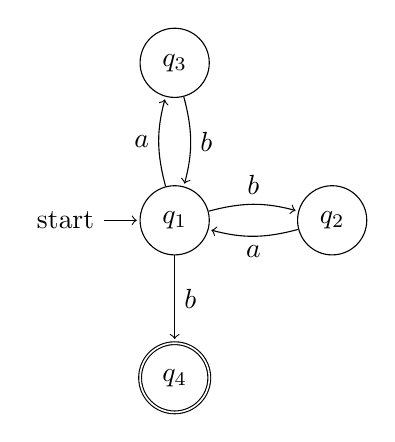
\begin{tikzpicture}[shorten >=1pt,node distance=2cm,on grid,auto] 
    \node[state,initial] (1) {$q_1$};
    \node[state] (2) [right=of 1] {$q_2$};
    \node[state] (3) [above=of 1] {$q_3$};
    \node[state,accepting] (4) [below=of 1] {$q_4$};
    \path[->]
        (1) edge [bend left=15] node {$b$} (2)
            edge [bend left=15] node {$a$} (3)
            edge node {$b$} (4)
        (2) edge [bend left=15] node {$a$} (1)
        (3) edge [bend left=15] node {$b$} (1);
    \end{tikzpicture}
\end{center}

\subsection*{Pumping lemma for regulære sprog}

Pumping lemmaet kan benyttes til at bevise at et sprog \textit{ikke} er regulært. \\

\textbf{Thm.} Hvis $A$ er et regulært sprog så $\exists p$ (pumpe-længde) s.t. hvis $s \in A$ og $|s|\ge p$ så kan $s$ deles op i tre dele $s=xyz$ således at $s$ tilfredsstiller:
\begin{enumerate}
    \item $\forall i \ge 0: xy^i z \in A$
    \item $|y|>0$
    \item $|xy| \le p$
\end{enumerate}

\textbf{Bevis.} Lad $M=(Q, \Sigma, \delta, q_0, F)$ være en DFA med $L(M)=A$ og lad pumpe-længden $p=|Q|$. Vi vælger en vilkårlig streng $s \in A$, hvor $|s|=n\ge p$. Når $M$ læser $s$ vil der altså være $n$ præcis $n$ state-transitions og derfor vil sekvensen af states som $M$ befinder sig i mens $s$ læses have længde $n+1$ (pga. vi er i state $q_0$ før det første symbol i $s$ læses). Da $|Q| = n$ følger det af pigeonhole princippet at $\exists q \in Q$ s.t. $q$ besøges mindst to gange i løbet af læsningen af $s$. Illustration:    
\begin{center}
	\includegraphics[width=0.65\textwidth]{pumpingLemma.JPG}
\end{center}
Som det kan ses på tegningen, kan vi skrive $s=xyz$, hvor $x$ er den del af $s$ som er indtil den state som gentages; $y$ er den del mellem states der gentages; $z$ er den del efter gentagelsen. \\

Opfyldelse af betingelserne: 
\begin{enumerate}
	\item Det er åbenlyst fra illustrationen at `løkken' fra og til den gentagne state kan gennenmløbes et vilkårligt antal gange (inkl. 0 gange). 
	\item $|y|>0$ fordi `løkken' angiver en sekvens, der finder sted mellem to \textit{forskellige} forekomster af den gentagne state. (Bemærk at $|y|>0$ også gælder hvis sekvensen er er $\ldots q_9q_9 \ldots$, altså et self-loop uden mellemliggende states). 
	\item Følger af pigeonhole princippet fordi de første $p+1$ states må indeholde en gentagen state da $p=|Q|$.    
\end{enumerate} 
\begin{flushright}
	\qed
\end{flushright}

\subsection*{Eksempel: Anveldelse af pumping lemmaet}

Vi vil vise at $L=\{a^{k^{2}}| \; k \ge 0\}$ ikke er regulært v.h.a. pumping lemmaet. \\

Antag til modstrid at $L$ er regulært. Lad $p$ være pumpe-længden. Vælg $s=a^{p^{2}} \in L$. Da $|s|=p^2 \ge p$ kan vi skrive $s=xyz$. Men hvis vi betragter $s'=xy^2z$ ser vi at $|s'| \le p^2 + p < p^2+2p+1=(p+1)^2$. Den første ulighed holder fordi $|y| \le p$. Det følger at $s' \notin L$, hvilket er en modstrid, der viser at $L$ ikke er regulært. 
\begin{flushright}
	\qed
\end{flushright}    


\newpage 
\section{Pushdown automata and context-free languages}

\subsection*{Outline}
\begin{itemize}
	\item Definition af context-free grammars og -sprog
	\item Definition af pushdown automata 
	%\item Bevis-skitse over ækvivalens af context-free languages og pushdown automata 
	\item Eksempel på context-free sprog og pushdown automata
	\item Bevis for Pumping lemmaet for context-free sprog
	\item Eksempel på anvendelse af pumping lemmaet
\end{itemize}

\subsection*{Context-free grammars og -sprog}

En context-free grammar (CFG) $M$ defineres som $M=(V, \Sigma, R, S)$, hvor 
\begin{itemize}
	\item $V$: variabler
	\item $\Sigma$: Terminal symbols. NB: $\Sigma \cap V = \emptyset$ 
	\item $R$: Substitutions-regler
	\item $S \in S$: start-variabel 
\end{itemize}

Et sprog $L$ er context-free (CFL), hvis det genereres af en CFG. \\

\textbf{Eksempel.} Lad $M=(\{S\}, \{0,1\},R, S)$, hvor $R$ er givet ved
\begin{align*}
	&S \rightarrow SS \; | \; 0 \; | \; 1
\end{align*}
være en CFG. Vi kan fx derive strengen 0011 (leftmost derivation): 
\begin{align*}
S \rightarrow SS \rightarrow \rightarrow SSS \rightarrow SSS \rightarrow 0SSS \rightarrow 00SS \rightarrow 001S \rightarrow 0011
\end{align*}

\subsection*{Pushdown automata}

En (non-deterministisk) pushdown automaton $N$ kan defineres som en NFA med en stack, d.v.s. $N=(Q, \Sigma, \Gamma, \delta, q_0, F)$, hvor
\begin{itemize}
	\item $Q$: states
	\item $\Sigma$: alfabet 
	\item $\Gamma$: stack-alfabet 
	\item $\delta$: transitionsfunktion, $Q \times \Sigma_{\varepsilon} \times \Gamma_{\varepsilon} \rightarrow \mathcal{P}(Q \times \Gamma_{\varepsilon})$
	\item $q_0$: start state
	\item $F$: accept states 
\end{itemize}

\textbf{Thm.} Et sprog $A$ er kontekstfrit $\Leftrightarrow$ $\exists$ pushdown automaton $M$ s.t. $L(M)=A$. (Bevises ikke). \\

\textbf{Eksempel.} Lad $L=\{w\in \{a,b,c\}^*| \; \#_a(w) =\#_b(w)\}$. $L$ er et CFL fordi den følgende pushdown automaton $N=(\{q_0,q_1,q_2\}, \{a,b,c\}, \{a,b,\$\}, \delta, q_0, \{q_2\})$ har $L(N)=L$:

\begin{center}
	\begin{tikzpicture}[shorten >=1pt,node distance=4cm,on grid,auto] 
	\node[state,initial] (q0) {$q_0$};
	\node[state] (q1) [right=of q0] {$q_1$};
	\node[state,accepting] (q2) [below=of q1] {$q_2$};
	\path[->]
	(q0) edge node {$\varepsilon,\varepsilon \rightarrow \$$} (q1)
	(q1) edge [align=left,loop right] node {$a,\varepsilon \rightarrow a$\\$a,b \rightarrow \varepsilon$\\$b,\varepsilon \rightarrow b$\\$b,a\rightarrow \varepsilon$\\$c,\varepsilon \rightarrow \varepsilon$} ()
	edge node {$\varepsilon, \$ \rightarrow \varepsilon$} (q2);
	\end{tikzpicture}
\end{center} 


\subsection*{Pumping lemma for context-free sprog}

Hvis $A$ er et CFL, så er det et tal $p$ (pumpe-længde) hvor, hvis $s \in A$ og $|s| \ge p$, så kan $s$ opdeles i 5 stykker, $s=uvxyz$, s.t. de følgende 3 betingelser tilfredsstilles: 
\begin{itemize}
	\item $\forall i \ge 0: uv^ixy^iz \in A$
	\item $|vy| > 0$
	\item $|vxy| \le p$. 
\end{itemize} 

\textbf{Bevis.} Lad $A$ være et CFL og $G$ være en CFG med $L(G)=A$. Lad $b$ være det maksimale antal symboler på højresiden af en regel i $G$. Det følger at en node i et vilkårligt parse tree (PT) opnået v.h.a. $G$ kan have $\le b$ børn, d.v.s. der er $\le b$ blade 1 trin fra roden, $\le b^2$ blade 2 trin fra roden etc. Det følger, at hvis højden på et PT er $\le h$ så er længden på den udledede streng (d.v.s. antal blade i PTet) $\le b^h$, og omvendt, hvis der er $\ge b^h+1$ blade i PTet, så er det $\ge h+1$ højt. \\

Lad pumpe-længden $p=b^{|V|+1}$. Det følger at enhver streng $s \in A$, hvor $|s| \ge p$ har et PT, der er $\ge |V|+1$ højt fordi $b^{|V|+1} \ge b^{|V|}+1$. Betragt nu en vilkårlig streng $s$ som opfylder førnævnte. Lad $T$ være ét PT\footnote{Hvis grammatiken $G$ er ambiguous, vælg da det $T$ som udleder $s$ v.h.a. færrest muligt antal nodes.} der udledes $s$ fra $G$. $T$ er mindst $|V|+1$ højt (d.v.s. længste sti fra rod til blad) og indeholder mindst $|V|+2$ noder på denne længste rod-til-blad-sti. Bladet på denne sti er et terminal-symbol\footnote{Det er blade i PTer altid per definition.}, så $|V|+1$ af disse er symboler fra $V$. Det følger at $\exists R \in V$ som gentages på denne sti jf. pigeonhole princippet. Dette kan illustreres således:
\begin{center}
	\includegraphics[width=0.65\textwidth]{pumpingLemmaCFL.JPG}
\end{center}
Illustrationen viser også inddelingen af $s$ i $uvxyz$. \\

Opfyldende af betingelserne:
\begin{enumerate}
	\item Da begge subtrees af $R$ er dannet af samme variabel kan de erstattes med hinanden uden videre. Ved at sætte det større subtree ind på det lille subtrees plads (evt. gentagne gange) kan strengene $uv^ixy^iz$ for $i>1$ opnås (nederste billede t.v.). Ved at sætte det lille subtree ind på det større subtrees plads opnås strengen $uv^0xy^0z=uxz$ (nederste billede t.h.). Så erstatningen er altså gyldig $\forall i \ge 0$.
	\item $|vy|=0$ hvis $v=y=\varepsilon$. Hvis dette er tilfældet kan det større subtree sættes ind på det mindre subtrees plads og derved give et $T'$ der også udleder $s$ men indeholder færre nodes end $T$ (tænk på det ift. nederste billede t.h.; dette PT ville stadig generere $s$). Dette er en modstrid fordi $T$ er det parse tree med mindst mulige antal nodes. Det følger at betingelsen er opfyldt.
	\item Vi sørger for at vælge $R$ s.t. de to gentagelser forekommer blandt de nederste $|V|+1$ variabler i $T$. Så det subtree $vxy$ som $R$ udleder kan have længde $ \le b^{|V|+1}=p$.     
\end{enumerate}
\begin{flushright}
	\qed
\end{flushright}
\subsection*{Eksempel: Anvendelse af pumping lemmaet}

Vi vil vise at $L=\{a^n b^n c^n| \; n \ge 0\}$ ikke er et CFL v.h.a. pumping lemmaet. \\

Antag til modstrid at $L$ er et CFL. Lad $p$ være pumpe-længden (se beviset ovenfor). Vælg strengen $s=a^p b^p c^p \in L$. Da $|s| \ge p$ kan vi skrive $s=uvxyz$ jf. pumping lemmaet. Lad $s'=uv^2xy^2z$. Vi ved at mindst én af $v$ og $y$ er ikke-tom jf. betingelse 2 i pumping lemmaet. Følgende to cases skal betragtes:
\begin{enumerate}
	\item Hvis både $v$ og $y$ kun består af ét alfabet-symbol (ikke nødvendigvis det samme): Da må det være tilfældet at $s' \notin L$ fordi det er mindst et og højest  to af alfabet-symbolerne, hvis antal øges.
	\item Hvis enten $v$ eller $y$ består af to alfabet-symboler (de kan ikke begge bestå af to alfabet-symboler jf. betingelse 3 i pumping lemmaet): Da må det være tilfældet at $s' \notin L$ fordi $s'$ indeholder alfabet-symboler, der ikke er i korrekt rækkefølge.   
\end{enumerate} 
D.v.s. at en modstrid er uundgåelig så $L$ er ikke et CFL.
\begin{flushright}
	\qed
\end{flushright}

\newpage
\section{Turing machines}

\subsection*{Outline}

\begin{itemize}
	\item Definition af Turing Maskine (TM) og Church-Turing tesen
	\item Multitape TMs og bevis for disses ækvivalens med single tape TMs
	\item Non-deterministiske TMs og bevis for disses ækvivalens med single tape TMs
	\item Definition af Turing decidability og -recognizability
	\item Eksempler på et decidable language med udgangspunkt i deres deciders
\end{itemize}

\subsection*{TMs og Church-Turing tesen}

TMs er abstrakte modeller af en computer med et ubegrænset mængde hukommelse; god abstraktion over en computer som vi kender den. \textit{Church-Turing tesen} formaliserer dette: ``Enhver funktion, der er beregnelig kan beregnes af en TM''. \\

En deterministisk single-tape TM $M$ er defineret som $M=(Q,\Sigma,\Gamma,\delta,q_0,q_{accept},q_{reject})$, hvor
\begin{itemize}
	\item $Q$: states
	\item $\Sigma$: input-alfabet, hvor $\sqcup \notin \Sigma$) 
	\item $\Gamma$: tape-alfabet, hvor $\sqcup \in \Gamma$ og $\Sigma \subseteq \Gamma$
	\item  $\delta$: transitionsfunktion, $Q \times \Gamma \rightarrow Q \times \Gamma \times \{L,R\}$
	\item $q_0$: start state
	\item $q_{accept}$: accept state
	\item $q_{reject}$: reject state (NB: $q_{accept} \ne q_{reject}$)
\end{itemize} 
En TM $M$ består af et læsehoved og et stykke tape (hukommelse) der strækker sig uendeligt til højre. Et input af længde $n$ skrives på de første $n$ pladser på tapen. Læsehovedet læser det første symbol og $\delta$ dikterer så (1) hvilken state $M$ skal skifte til, (2) hvilket symbol der skal skrives på tapen og (3) hvilken retning læsehovedet skal bevæge sig ét trin i. \\

\subsection*{Multitape TMs.} 

Mange afarter af TMs, fx en TM med et vilkårligt (men fixed) antal tapes. $\delta$ for en TM $M$ med $k$ tapes kan skrives som $\delta: Q \times \Gamma^k \rightarrow Q \times \Gamma^k \times \{L,R\}^k$. D.v.s. $M$ er stadig kun i ét state af gangen men arbejder simultant på $k$ tapes, der hver har ét læsehoveds. \\

\textbf{Thm.} Enhver multitape TM har en ækvivalent single-tape TM.\\

\textbf{Bevis.} Lad $M$ være en $k$-tape TM og lad $N$ være en 1-tape TM. Vi kan simulere $M$ på $N$ ved at gøre følgende på input $s=w_1w_2 \cdots w_n$:
\begin{enumerate}
	\item Formatér $N$ tape således: $\underline{\#}\stackrel{\bullet}{w_1}w_2\cdots w_n \#\stackrel{\bullet}{\sqcup}\# \cdots \#$. Prikkerne over symbolerne viser de virtuelle læsehoveders placering og understregningen viser det faktiske læsehoveds placering.
	\item Scan inputtet fra det første $\#$ til det $(k+1)$ste (d.v.s. sidste) $\#$ for at bestemme tape-indholdet under de $k$ virtuelle læsehoveder. Scan inputtet fra det $(k+1)$ste $\#$ til det første $\#$ og opdater tape-indholdet og flyt de virtuelle læsehoveder i overensstemmelse med $\delta$ for $M$. 
	\item Hvis et virtuelt læsehoved flyttes til venstre ud på et $\#$ behold det da på det forhenværende symbol; dette svarer til at læsehovedet forsøger at rykke ud over venstresiden af tapen. Hvis et virtuelt læsehoved flyttes til højre ud på et $\#$ så flyt da hele tapeindholdet fra og med det pågældende $\#$ én plads til højre (right shift) og indsæt et $\sqcup$ på den nye tomme plads, hvor det virtuelle læsehoved så placeres over; dette svarer til at læsehovedet rykker ud på den tomme del af tapen til højre som er uendelig.  
\end{enumerate}
\begin{flushright}
	\qed
\end{flushright}

\subsection*{Non-deterministiske TMs}

En non-deterministisk TM er en TM, hvor TMen i hvert trin af beregningen kan følge forskellige muligheder (ligesom en NFA). Derved opnås en træstruktur, hvor hver gren repræsenterer en mulig beregning for TMen. Altså har vi en transitionsfunktion 
$$\delta: Q \times \Gamma \rightarrow \mathcal{P}(Q \times \Gamma \times \{L,R\})$$
Hvis en gren ender i $q_{accept}$ så accepteres inputtet. \\

\textbf{Thm.} Enhver non-deterministisk TM har en ækvivalent deterministiske TM. \\

\textbf{Bevis.} Lad $N$ være en vilkårlig non-deterministisk TM. Lad $D$ være en 3-tape deterministisk TM (der eksisterer en ækvivalent 1-tape TM jf. Thm. vist ovenfor). Vi viser Thm. ved at vise at $N$ kan simuleres på $D$. \\

Indholdet på $D$s tre tapes er:
\begin{itemize}
	\item Tape 1: Input strengen. Ændres aldrig.
	\item Tape 2: Simulations-tape.
	\item Tape 3: Adresse-tape.
\end{itemize}  
Vi betragter $N$s beregningstræ. Enhver node i dette træ kan have højest $b$ børn, hvor $b$ er det maksimale antal muligheder givet i $\delta$ for $N$. Enhver node får tildelt et navn over alfabetet $\Gamma_b=\{1,2,\ldots,b\}$. Fx så angiver adressen 231 at vi tager rodens 2. barn, denne nodes 3. barn og denne nodes 1. barn. Hvis en adresse ikke svarer til en node så ignoreres denne adresse og den næste adresse behandles. Så det vi faktisk laver svarer til BFS på $N$s beregningstræ.\footnote{Bemærk at DFS ikke egner sig her, da denne algoritme traverserer grenene én af gangen. Så hvis en gren er et uendeligt loop (og dermed uendelig lang) vil DFS aldrig blive færdig med at gennemløbe beregningstræet.} Beregningstræets rod har adressen $\varepsilon$. \\

Vi kan nu beskrive hvad $D$ gør på input $\langle N, w \rangle$:
\begin{enumerate}
	\item Kopier indholdet af tape 1 til tape 2 og skriv $\varepsilon$ til tape 3. 
	\item Simuler $N$ på indholdet af tape 2. Før hvert trin i $N$ konsulteres tape 3 for at vide, hvilket valg der skal tages ift. $N$s $\delta$. Hvis der på tape 3 læses et $\sqcup$ \textit{eller} hvis der ikke er noget valg for $\delta$ der svarer til adressen på tape 3 \textit{eller} hvis grenen ender i $q_{reject}$ \textit{så} gå til trin 3. Hvis grenen ender i $q_{accept}$ så accepter. 
	\item Erstat strengen (tallet) på tape 3 med den næste streng (tal) i rækken og gentag trin 2 og 3. 
\end{enumerate}
\begin{flushright}
	\qed
\end{flushright}

\subsection*{Turing recognizability og decidability}

\textbf{Recognizable.} En sprog $L$ er Turing recognizable (genkendeligt) hvis der eksisterer en TM $M$ s.t. hvis $s \in L$ så accepteres $s$ af $M$. \\ 

\textbf{Decidable.} Et sprog $L$ er Turing decidable (afgørligt), hvis der eksisterer en TM $M$ s.t. $M$ accepterer en $s$ hvis og kun hvis $s \in L$. (Bemærk at hvis et sprog er recognizable er det også decidable men ikke vice versa.)\\

\subsubsection*{Eksempel 1} % Udelad eventuelt.

Lad $A_{DFA} =\{\langle B,w \rangle| \; B \text{ er en DFA der accepterer input streng } w\}$. \\

\textbf{Thm.} $A_{DFA}$ er decidable. \\

\textbf{Bevis.} Vi beviser Thm. ved at give en konkret TM $M$ som decider $A_{DFA}$. \\

Lad $M$ være en TM der på input $\langle B, w \rangle$ gør følgende: 
\begin{enumerate}
	\item Simuler $B$ v.h.a. $M$
	\item Giv $w$ som input til $B$. Hvis $B$ ender i et accept state, så accept. Hvis $B$ ikke ender i et accept state så reject. 
\end{enumerate}

\subsubsection*{Eksempel 2}

Vi vil konstruere en TM der beregner funktionen $f(w)=(ww)^{\mathcal{R}}$. \\

Lad $M$ være en 2-tape TM der gør det følgende på input $w$: 
\begin{enumerate}
	\item Hvis det første symbol i $w$ er $\sqcup$ så er $w=\varepsilon$, så $M$ accepterer. Ellers fortsæt. 
	\item Kopier $w$ til tape 2 ved at skrive symbolerne fra tape 1 ét af gangen indtil et $\sqcup$ læses på tape 1. 
	\item Flyt tape 1s læsehoved til symbolet længst til venstre. Flyt tape 1s læsehoved til det første $\sqcup$ (d.v.s. én plads til højre).
	\item Gentag trin 2 én gang. (Nu indeholder tape 2 $ww$).
	\item Flyt tape 2s læsehoved til det første symbol $w_1$ og marker det så det bliver $\stackrel{\bullet}{w_1}$. 
	\item Flyt tape 1s læsehoved til det første symbol til venstre. 
	\item Flyt tape 2s læsehoved til det sidste symbol, d.v.s. det sidste non-$\sqcup$ symbol. (Dette er det sidste symbol i $ww$).
	\item Skriv indholdet fra tape 2 til tape 1. Gør dette ved at skrive et symbol, hvorefter tape 2s læsehoved flyttes én til venstre og tape 1s læsehoved flyttes én til højre. Fortsæt indtil og med at $\stackrel{\bullet}{w_1}$ (uden bullet-tegnet) er skrevet til tape 1.
	\item Flyt begge læsehoveder helt til venstre og accepter. 
\end{enumerate}





\newpage
\section{Decidability}

\subsection*{Outline}

\begin{itemize}
	\item Definition af decidability.
	\item Hvordan decidability bevises og eksempler 
	\item Definition af undecidability
	\item Hvordan undecidability bevises og eksempler  
\end{itemize}

\subsection*{Decidability}

Et sprog $L$ er Turing decidable (afgørligt), hvis der eksisterer en TM $M$ s.t. $M$ accepterer en $s$ hvis og kun hvis $s \in L$. (Bemærk at hvis et sprog er decidable er det også recognizable men ikke vice versa.)\\

\subsection*{At bevise decidability}

Hvis $L$ er et decidable sprog kan man vise at $L$ er decidable ved at konstruere en decider $M$ s.t. $L(M)=L$. \\ 

\subsubsection*{Eksempel 1}

Lad $L=\{\langle G,M \rangle| \; G \text{ er en CFG og } M \text{ er en DFA og } L(G) \cap L(M)=\emptyset \}$. \\

Følgende TM $N$ er en decider for $L$. På input $\langle G,M \rangle$ gør $M$ følgende:
\begin{enumerate}
	\item Konstruér en CFG $G'$ s.t. $L(G')=L(G) \cap L(M)$.\footnote{$G$ er et CFL og $M$ er et regulært sprog, så $L(G) \cap L(M)$ er et CFL.}
	\item Marker alle terminale symboler i $G'$.\footnote{Trin 2-4 svarer til $E_{CFG}$, se s. 199f i Sipser. I trinnene testes om startvariablen i $G'$ kan generere en streng af terminaler.}
	\item Gentag følgende indtil ingen nye variabler markeres:
	\begin{enumerate}
		\item Markér enhver variabel $A$ hvor $G'$ har en regel $A \rightarrow U_1 U_2 \cdots U_k$ og hvert symbol $U_1,U_2,\ldots,U_k$ allerede er markeret
	\end{enumerate}
	\item Hvis start variablen ikke er markeret, accept; eller reject. 
\end{enumerate} 

\subsubsection*{Eksempel 2}

Lad $L=\{\langle M, w \rangle |; M \text{ er en TM der tager } \le 1332 \text{ trin på input } w\}$.\\

Følgende 2-tape TM $N$ er en decider for $L$. På input $\langle M,w \rangle$ gør $M$ følgende: 
\begin{enumerate}
	\item Simulér $M$ på $w$ på tape 1 
	\item På tape 2 tælles antal trin taget af $M$ på tape 1 (antager at vi har binary adder til rådighed).
	\item Hvis $M$ accepts eller rejects \textit{og} tallet på tape 2 er højest 1332, accept. Hvis tallet på tape 2 bliver $>1332$ så reject.   
\end{enumerate} 

\subsection*{Undecidability}

\textbf{Thm.} Der eksisterer sprog, der ikke er Turing recognizable. \\

\textbf{Bevis.} Vi observerer først at kardinaliteten af mængden af TMs er tælleligt, uendelig. Lad $\Sigma=\{0,1\}$.\footnote{Alle TMs kan kodes i binær.} Vi har at $|\Sigma^*|=\aleph_0$ fordi der er et endeligt antal strenge af en given længde, så $\Sigma^*$ kan enumereres. Det er åbenlyst at $\Sigma^*$ rummer kodning af alle TMs (og mere til). Det følger at kardinaliteten af mængden af TMs er tælleligt, uendelig. \\

Vi viser nu at kardinaliteten af mængden af sprog er overtællelig. Her viser vi først mængden af uendelige binære sekvenser er overtællelig vha. Cantors diagonaliseringsmetode: \\

Hvis vi prøver at enumerere alle uendelige binære sevkenser er det altid muligt at finde en uendelig binær sekvens, der ikke er i enumerationen. Lad $b_i$ for $i \in \N$ være den $i$te sekvens i enumerationen. Vi konstruerer nu den uendelige bit-sekvens:
\[b_i'= \left\{ \begin{array}{ll}1 & \mbox{if $b_{i_i} = 0$};\\0 & \mbox{if $b_{i_i}=1$}.\end{array} \right. \] 
På denne måde er $b_i'$ forskellig fra $b_i$, $\forall i$ i mindst én position. Dette viser at mængden af uendelige binære sekvenser er overtællelig. \\

Ethvert sprog kan defineres vha. en karakteristisk sekvens over $\Sigma^*$, hvor $1$ indikerer medlemskab og $0$ indikerer ikke-medlemskab. En sådan karakteristisk sekvens er en uendelig bit-sekvens fordi $\Sigma^*$ er uendelig. Så mængden af alle sprog er en bijektion med mængden bestående af alle uendelig bit-sekvenser. Det følger at kardinaliteten af mængden af sprog er overtællelig. \\

Så der er tælleligt, uendelig mange TMs og overtælleligt (d.v.s. mange, mange flere!) sprog. Det følger at der eksisterer sprog, der ikke recognizes af nogen TM. \\
\begin{flushright}
	\qed
\end{flushright}

\textbf{Korr.} Der eksisterer sprog, der er undecidable. \\

\textbf{Bevis.} Følger af bevis for Thm. fordi hvis et sprog er unrecognizable er det også undecidable.   
\begin{flushright}
	\qed
\end{flushright}

\subsection*{At bevise undecidability}

Man kan enten bruge mapping reductions (vil ikke blive gjort her) eller modstridsbeviser. 

\subsubsection*{Eksempel 1}

Lad $A_{TM}=\{\langle M,w \rangle | \; M \text{ er en TM og } M \text{ accepterer } w\}$. \\

\textbf{Thm.} $A_{TM}$ er undecidable. \\

\textbf{Bevis.} Antag til modstrid at $H$ er en decider for $A_{TM}$. På input $\langle M, w \rangle$, hvor $M$ er en TM og $w$ er en streng gør $H$ følgende: 
\[H(\langle M, w\rangle)= \left\{ \begin{array}{ll} accept & \mbox{hvis $M$ accepts $w$};\\reject & \mbox{hvis $M$ ikke accepts $w$}.\end{array} \right. \] 
Lad $D$ være en ny TM der bruger $H$ som en subrutine til at afgøre, hvad $M$ gør når den får sig selv som input. $D$ gør følgende på input $\langle M \rangle$ ($D$ outputter altid det omvendte af $M$):
\[D(\langle M\rangle)= \left\{ \begin{array}{ll} accept & \mbox{hvis $M$ ikke accepts $\langle M \rangle$};\\reject & \mbox{hvis $M$ accepts $\langle M \rangle$}.\end{array} \right. \] 
Nu giver vi $D$ som input til sig selv, hvilket vil resultere i:
\[D(\langle D \rangle)= \left\{ \begin{array}{ll} accept & \mbox{hvis $D$ ikke accepts $\langle D \rangle$};\\reject & \mbox{hvis $D$ accepts $\langle D \rangle$}.\end{array} \right. \] 
Dette er åbenlyst en modstrid fordi lige meget hvad $D$ gør er den tvunget til at gøre det modsatte. Derfor kan hverken $H$ (eller $D$) kan eksistere og det følger at $A_{TM}$ er undecidable. 
\begin{flushright}
	\qed
\end{flushright}

\newpage
\section{Reducibility (including mapping reductions and polynomial reductions}

\subsection*{Outline}

\begin{itemize}
	\item Mapping reductions og polynomial time reductions, definitioner og formål
	\item NP-completeness definition og relation til polynomial time reductions
	\item Eksempler på polynomial time reductions til at vise at problem er NP-complete
\end{itemize}

\subsection*{Mapping reductions og polynomial time reductions}

\textbf{Mapping reductions.} Lad $A$ og $B$ være sprog. $A \le_m B$ hvis $\exists$ en beregnelig funktion $f: \Sigma^* \rightarrow \Sigma^*$, hvor $\forall w: (w \in A \Longleftrightarrow f(w) \in B)$. Vi kalder $f$ reduktionen fra $A$ til $B$. \\

\textit{Formål:} Bevise (un-)decidability. Hvis $A \le_m B$ og $B$ er decidable, så er $A$ decidable. Og hvis $A \le_m B$ og $A$ er undecidable, så er $B$ undecidable. \\

\textbf{Polynomial time reductions.} Lad $A$ og $B$ være sprog. $A \le_p B$ hvis $\exists$ en funktion $f: \Sigma^* \rightarrow \Sigma^*$ der kan beregnes i polynomiel tid, hvor $\forall w: (w \in A \Longleftrightarrow f(w) \in B)$. Vi kalder $f$ polynomial-time reduktionen fra $A$ til $B$. \\

\textit{Formål:} Essentielt værktøj til at vise at et problem er NP-complete (NPC). Hvis $B \in NPC \wedge B \le_p C \wedge C \in NP \Longrightarrow C \in NPC$.


\subsection*{NP-completeness og polynomial time reductions: HAMCYCLE}

Som et eksempel på en polynomial time reduction vil jeg nu vise, at hamiltonian cycle er NP-complete vha. en polynomial time reduction. \\

\textbf{Definition af NP-complete.} $A \in NP \wedge \forall B \in NP: (B \le_p A) \Longrightarrow A \in NPC$. \\

\textbf{Hamiltonian Cycle problemet (HAMCYCLE):} Lad $G=(V,E)$ være en uorienteret graf. $G$ indeholder en HAMYCYCLE iff. $\exists$ en simple cycle\footnote{Cycle hvor kun én vertex gentages; alle andre vertices indgår præcis én gang.} i $G$ der indeholder alle $v \in V$. \\

\textbf{Thm.} HAMCYCLE $\in NPC$. \\

\textbf{Bevis.} Til beviset skal vi bruge VERTEX-COVER\footnote{Et vertex cover er en mængde af vertices i en uorienteret graf s.t. alle edges er incidente til mindst én vertex i vertex coveret.} $\in NP$. \\

Først viser vi at HAMCYCLE $\in NP$. Et certifikat $c$ er en sekvens af $|V|$ vertices i $G$. Vi tjekker (1) at $c$ indeholder alle $v \in V$, (2) at sekvensen former en cycle og (3) at cyclen er en simple cycle. Dette kan åbenlyst gøres i polynomiel tid så HAMCYCLE $\in NP$. \\

Nu viser vi VERTEX-COVER $\le_p$ HAMCYCLE. \\

 uorienteret graf $G=(V,E)$ og et $k \in \Z^+$ (størrelse af vertex cover) konstruerer vi en graf $G'=(V',E')$, der har en HAMCYCLE iff. $G$ har et VERTEX-COVER af størrelse $k$. \\

For at konstruere $G$ bruger vi en widget -- mere præcist vil $G'$ indeholde præcis én widget for hver edge $(u,v) \in E$. (a) viser en widgets opbygning og navngivning af de 12 vertices heri. (b)-(d) viser de eneste tre mulige måder at traversere de 14 edges i en widget på:
\begin{center}
	\includegraphics[width=\textwidth]{widget.PNG}
\end{center}
Desuden inkluderer vi $k$ selector-vertices, hvor $k$ er størrelsen på $G$s VERTEX-COVER. For at konstruere $G'$ fra $G$ vha. widgets gøres følgende to trin:
\begin{enumerate}
	\item For alle vertices $v \in V$ laves der en arbitrær ordning af de tilstødende knuder. Hvis vi har en knude $w$ og den er indident til $(x,y,z)$ så tilføjes kanterne $([w,x,6],[w,y,1])$ og $([w,y,6],[w,z,1])$.
	\begin{enumerate}
		\item Intuitionen bag disse edges er at hvis vi vælger en $v \in V$, der er del af $G$s VERTEX-COVER, så vil vi kunne lave en sti i $G'$ der dækker (covers) alle de widgets der repræsenterer edges, der er incidente til $v$.
	\end{enumerate} 
	\item De to endeknuder i stierne fra trin 1 forbindes til alle selector vertices. Bemærk at hvis en sti fx ender i $[u,v,6|$ er det den modsatte side af ``pinden'', altså $[u,v,1]$, der skal forbindes til selector-verticen (og vice versa hvis stien ender i $[u,v,1]$).  
\end{enumerate}
Nedenstående er et simpelt eksempel, hvor $G'$ konstrueres ud fra $G$. Lad $G$ være ($x$ og $y$ er markeret fordi disse udgør $G$s VERTEX-COVER): 
\begin{center}
	\includegraphics[width=0.50\textwidth]{graph1.JPG}
\end{center}
Der er tre edges i $G$ og to knuder i $G$s vertex cover så skelettet til $G'$ vil se sådan ud: 
\begin{center}
	\includegraphics[width=0.75\textwidth]{widget1.JPG}
\end{center}
Vi beslutter os for at ordne nabo-vertices til alle vertices i $G$ således (arbitrært):
\begin{align*}
	&\text{adj}(x)=(y,z) \\	
	&\text{adj}(y)=(x,z) \\
	&\text{adj}(z)=(x,y)
\end{align*}
Derfor tegner vi nu de følgende tre stier (sorte kanter): 
\begin{center}
	\includegraphics[width=0.80\textwidth]{widget2.JPG}
\end{center}
Nu forbinder vi sti-enderne til selector-vertices $S_1$ og $S_2$ (blå kanter) og får den færdige $G'$: 
\begin{center}
	\includegraphics[width=0.80\textwidth]{widget3.JPG}
\end{center}
Nu viser vi at $G'$ er polynomiel i størrelsen af $G$. Bagefter viser vi at det er en gyldig reduktion fra VERTEX-COVER til HAMCYCLE. Altså alt i alt at ovenstående er en polynomial time reduction! \\

Følgende gælder for $|V'|$:
\begin{align*}
	|V| =& 12|E| + k && \text{(Fordi der er 12 vertices pr. widget)} \\
	\le& 12|E| + |V|  && (\text{Fordi } k \le |V| \text{ da det er størrelsen af et vertex cover})
\end{align*}
Følgende gælder for $|E'|$: For det første har hver widget $14|E|$ edges. Desuden er der følgende antal edges mellem widgets:
\begin{align*}	
	\sum_{u \in V} (\text{degree}(u)-1) = 2|E|-|V| && \text{(Følger af handshake thm.)} 
\end{align*}
Endelig har $G'$ 2 edges for hvert par af en $v \in V$ og en selector-vertex, d.v.s. $2k|V|$ edges. Dette skyldes at de stier, der blev konstrueret (og som hver har to edges til hver selector vertex) kan ses som en \textit{vertex} i $G$.\footnote{Intuitive giver det god mening, men er ikke 100p skarp på, hvorfor det er tilfældet.} Dette givet alt i alt: 
\begin{align*}
	|E'| =& 14|E|+(2|E|-|V|)+(2k|V|) \\
	=& 16|E|+2k|V|-|V| \\
	=& 16|E|+2(k-1)|V| \\
	\le& 16|E|+(2|V|-1)|V| 
\end{align*}
Så både $G'$ er polynomiel i størrelsen af $G$ da $|V'|$ og $|E'|$ er polynomielle i størrelserne af $|V|$ og $|E|$. \\

Nu mangler vi kun at vise, at ovenstående er en gyldig reduktion af VERTEX-COVER til HAMCYCLE. \\

\textit{Viser:} $G$ har VERETEX-COVER af størrelse $k$ $\Longrightarrow$ $G'$ har en HAMCYCLE. \\

Antag at $G$ har et VERTEX-COVER $V^* \subseteq V$ af størrelse $k$ og at $V^*=\{u_1,\ldots,u_k\}$. I $G'$ markeres følgende edges: \footnote{Bemærk at vi følger CLRS og betragter en HAMCYCLE som bestående af edges, selvom en HAMCYCLE teoretisk set består af vertices}
\begin{enumerate}
	\item Start i $S_1$ og besøg første $u_1$. 
	\item Besøg fra $u_1$ alle widgets, der svarer til edges, der er indidente til $u_1$. 
	\item Gentag trin 1-2 for $u_2,\ldots,u_k$ og slut tilbage i $S_1$. 
	\item Tegn edges inde i widgets'ne.  
\end{enumerate} 
Dette resulterer i en HAMCYCLE i vores eksempel (blå bølger på edges i HAMCYCLE):
\begin{center}
	\includegraphics[width=0.75\textwidth]{widget4}
\end{center}
Da $V^*$ er et VERTEX-COVER for $G$ er hver edge $e \in E$ incident til en $v \in V^*$. Derfor besøger cyclen hver widget i $G'$. Cyclen besøger også hver selector vertex, samt $S_1$ 2 gange, så det er en HAMCYCLE. \\

\textit{Viser:} $G'$ har HAMCYCLE $\Longrightarrow$ $G$ har et VERTEX-COVER. \\

Antag at $G'$ har en HAMCYCLE $C \subseteq E'$. Vi kan indse at $G$ må indeholde et VERTEX-COVER ved at betragte følgende gennemløb af $G'$:
\begin{enumerate}
	\item Start i $S_1$ og lav et maximal path gennemløb (d.v.s. længste mulige gennemløb), hvor der ikke indgår en anden selector vertex $S_j$. Stop når en anden selector vertex nås. Dette kalder vi en ``cover path'' 
	\begin{enumerate}
		\item På tegningen er der en markeret kant fra $S_1$ til $[x,y,1]$, hvorfor $x$ er i $G$s VERTEX-cover da man med denne fremgangsmåde dækker (coverse) alle kanter som er incidente til $x$ i $G$.
	\end{enumerate} 
	\item Lav tilsvarende cover paths for alle andre selector vertices. Dette giver samme konklusion som i (a) bare for andre $v \in V$.  
\end{enumerate}
Alle widgets indgår i mindst én og højst to cover path jf. antagelsen om at $G'$ har en HAMCYCLE. Hvis en widget indgår i præcis én cover path (som det er tilfældet for $W_{xz}$ og $W_{yz}$ i det anvendte eksempel) så er den tilsvarende edge i $G$ dækket (covered) at den $v \in V$, hvis cover path det er. Hvis en widget indgår i to cover paths (som det er tilfældet for $W_{xy}$ i det anvendte eksempel) så er den tilsvarende edge i $G$ dækket af de to $u,v\in V$, hvis cover paths det er. 
\begin{flushright}
	\qed
\end{flushright}
\newpage
\section{NP-completeness proofs -- examples}

\subsection*{Outline}

\begin{enumerate}
	\item Definition af NP-complete 
	\item Hvordan man viser at noget er NP-complete (NPC) -- polynomial time reductions
	\item Bevis for at HAMCYCLE $\in NPC$
\end{enumerate}

\subsection*{NP-completeness}

\textbf{Definition af NP-complete.} $A \in NP \wedge \forall B \in NP: (B \le_p A) \Longrightarrow A \in NPC$. \\

\textit{Hvorfor interessant kompleksitetsklasse:} To grunde:
\begin{enumerate}
	\item Teoretisk: Hvis man kan vise at et problem $\in NPC$ kræver mere end polynomiel tid, så gør alle problemer i $NPC$ det i hvilket tilfælde $P \ne NP$.
	\item Praktisk: Hvis et problem $\in NPC$ spilder man sandsynligvis sin tid, hvis man prøver at finde på en polynomiel algoritme da der er bred tro på (omend ikke vished for) at $P \ne NP$.  
\end{enumerate}

\subsection*{Hvordan man beviser at et problem er i NPC}

\begin{enumerate}
	\item Vis at problem i NP (typisk nemt). 
	\item Vis at alle problemer i NP kan reduceres til nærværende problem i polynomiel tid (typisk sværere) -- d.v.s. vis at problem er NP-hard. Se nedenfor. 
\end{enumerate}

\textbf{Polynomial time reductions.} Lad $A$ og $B$ være sprog. $A \le_p B$ hvis $\exists$ en funktion $f: \Sigma^* \rightarrow \Sigma^*$ der kan beregnes i polynomiel tid, hvor $\forall w: (w \in A \Longleftrightarrow f(w) \in B)$. Vi kalder $f$ polynomial-time reduktionen fra $A$ til $B$. 

\subsection*{Bevis for at HAMCYCLE $\in NPC$}

\textbf{Hamiltonian Cycle problemet (HAMCYCLE):} Lad $G=(V,E)$ være en uorienteret graf. $G$ indeholder en HAMYCYCLE iff. $\exists$ en simple cycle\footnote{Cycle hvor kun én vertex gentages; alle andre vertices indgår præcis én gang.} i $G$ der indeholder alle $v \in V$. \\

\textbf{Thm.} HAMCYCLE $\in NPC$. \\

\textbf{Bevis.} Til beviset skal vi bruge VERTEX-COVER\footnote{Et vertex cover er en mængde af vertices i en uorienteret graf s.t. alle edges er incidente til mindst én vertex i vertex coveret.} $\in NP$. \\

Først viser vi at HAMCYCLE $\in NP$. Et certifikat $c$ er en sekvens af $|V|$ vertices i $G$. Vi tjekker (1) at $c$ indeholder alle $v \in V$, (2) at sekvensen former en cycle og (3) at cyclen er en simple cycle. Dette kan åbenlyst gøres i polynomiel tid så HAMCYCLE $\in NP$. \\

Nu viser vi VERTEX-COVER $\le_p$ HAMCYCLE. \\

uorienteret graf $G=(V,E)$ og et $k \in \Z^+$ (størrelse af vertex cover) konstruerer vi en graf $G'=(V',E')$, der har en HAMCYCLE iff. $G$ har et VERTEX-COVER af størrelse $k$. \\

For at konstruere $G$ bruger vi en widget -- mere præcist vil $G'$ indeholde præcis én widget for hver edge $(u,v) \in E$. (a) viser en widgets opbygning og navngivning af de 12 vertices heri. (b)-(d) viser de eneste tre mulige måder at traversere de 14 edges i en widget på:
\begin{center}
	\includegraphics[width=\textwidth]{widget.PNG}
\end{center}
Desuden inkluderer vi $k$ selector-vertices, hvor $k$ er størrelsen på $G$s VERTEX-COVER. For at konstruere $G'$ fra $G$ vha. widgets gøres følgende to trin:
\begin{enumerate}
	\item For alle vertices $v \in V$ laves der en arbitrær ordning af de tilstødende knuder. Hvis vi har en knude $w$ og den er indident til $(x,y,z)$ så tilføjes kanterne $([w,x,6],[w,y,1])$ og $([w,y,6],[w,z,1])$.
	\begin{enumerate}
		\item Intuitionen bag disse edges er at hvis vi vælger en $v \in V$, der er del af $G$s VERTEX-COVER, så vil vi kunne lave en sti i $G'$ der dækker (covers) alle de widgets der repræsenterer edges, der er incidente til $v$.
	\end{enumerate} 
	\item De to endeknuder i stierne fra trin 1 forbindes til alle selector vertices. Bemærk at hvis en sti fx ender i $[u,v,6|$ er det den modsatte side af ``pinden'', altså $[u,v,1]$, der skal forbindes til selector-verticen (og vice versa hvis stien ender i $[u,v,1]$).  
\end{enumerate}
Nedenstående er et simpelt eksempel, hvor $G'$ konstrueres ud fra $G$. Lad $G$ være ($x$ og $y$ er markeret fordi disse udgør $G$s VERTEX-COVER): 
\begin{center}
	\includegraphics[width=0.50\textwidth]{graph1.JPG}
\end{center}
Der er tre edges i $G$ og to knuder i $G$s vertex cover så skelettet til $G'$ vil se sådan ud: 
\begin{center}
	\includegraphics[width=0.75\textwidth]{widget1.JPG}
\end{center}
Vi beslutter os for at ordne nabo-vertices til alle vertices i $G$ således (arbitrært):
\begin{align*}
&\text{adj}(x)=(y,z) \\	
&\text{adj}(y)=(x,z) \\
&\text{adj}(z)=(x,y)
\end{align*}
Derfor tegner vi nu de følgende tre stier (sorte kanter): 
\begin{center}
	\includegraphics[width=0.80\textwidth]{widget2.JPG}
\end{center}
Nu forbinder vi sti-enderne til selector-vertices $S_1$ og $S_2$ (blå kanter) og får den færdige $G'$: 
\begin{center}
	\includegraphics[width=0.80\textwidth]{widget3.JPG}
\end{center}
Nu viser vi at $G'$ er polynomiel i størrelsen af $G$. Bagefter viser vi at det er en gyldig reduktion fra VERTEX-COVER til HAMCYCLE. Altså alt i alt at ovenstående er en polynomial time reduction! \\

Følgende gælder for $|V'|$:
\begin{align*}
|V| =& 12|E| + k && \text{(Fordi der er 12 vertices pr. widget)} \\
\le& 12|E| + |V|  && (\text{Fordi } k \le |V| \text{ da det er størrelsen af et vertex cover})
\end{align*}
Følgende gælder for $|E'|$: For det første har hver widget $14|E|$ edges. Desuden er der følgende antal edges mellem widgets:
\begin{align*}	
\sum_{u \in V} (\text{degree}(u)-1) = 2|E|-|V| && \text{(Følger af handshake thm.)} 
\end{align*}
Endelig har $G'$ 2 edges for hvert par af en $v \in V$ og en selector-vertex, d.v.s. $2k|V|$ edges. Dette skyldes at de stier, der blev konstrueret (og som hver har to edges til hver selector vertex) kan ses som en \textit{vertex} i $G$.\footnote{Intuitive giver det god mening, men er ikke 100p skarp på, hvorfor det er tilfældet.} Dette givet alt i alt: 
\begin{align*}
|E'| =& 14|E|+(2|E|-|V|)+(2k|V|) \\
=& 16|E|+2k|V|-|V| \\
=& 16|E|+2(k-1)|V| \\
\le& 16|E|+(2|V|-1)|V| 
\end{align*}
Så både $G'$ er polynomiel i størrelsen af $G$ da $|V'|$ og $|E'|$ er polynomielle i størrelserne af $|V|$ og $|E|$. \\

Nu mangler vi kun at vise, at ovenstående er en gyldig reduktion af VERTEX-COVER til HAMCYCLE. \\

\textit{Viser:} $G$ har VERETEX-COVER af størrelse $k$ $\Longrightarrow$ $G'$ har en HAMCYCLE. \\

Antag at $G$ har et VERTEX-COVER $V^* \subseteq V$ af størrelse $k$ og at $V^*=\{u_1,\ldots,u_k\}$. I $G'$ markeres følgende edges: \footnote{Bemærk at vi følger CLRS og betragter en HAMCYCLE som bestående af edges, selvom en HAMCYCLE teoretisk set består af vertices}
\begin{enumerate}
	\item Start i $S_1$ og besøg første $u_1$. 
	\item Besøg fra $u_1$ alle widgets, der svarer til edges, der er indidente til $u_1$. 
	\item Gentag trin 1-2 for $u_2,\ldots,u_k$ og slut tilbage i $S_1$. 
	\item Tegn edges inde i widgets'ne.  
\end{enumerate} 
Dette resulterer i en HAMCYCLE i vores eksempel (blå bølger på edges i HAMCYCLE):
\begin{center}
	\includegraphics[width=0.75\textwidth]{widget4}
\end{center}
Da $V^*$ er et VERTEX-COVER for $G$ er hver edge $e \in E$ incident til en $v \in V^*$. Derfor besøger cyclen hver widget i $G'$. Cyclen besøger også hver selector vertex, samt $S_1$ 2 gange, så det er en HAMCYCLE. \\

\textit{Viser:} $G'$ har HAMCYCLE $\Longrightarrow$ $G$ har et VERTEX-COVER. \\

Antag at $G'$ har en HAMCYCLE $C \subseteq E'$. Vi kan indse at $G$ må indeholde et VERTEX-COVER ved at betragte følgende gennemløb af $G'$:
\begin{enumerate}
	\item Start i $S_1$ og lav et maximal path gennemløb (d.v.s. længste mulige gennemløb), hvor der ikke indgår en anden selector vertex $S_j$. Stop når en anden selector vertex nås. Dette kalder vi en ``cover path'' 
	\begin{enumerate}
		\item På tegningen er der en markeret kant fra $S_1$ til $[x,y,1]$, hvorfor $x$ er i $G$s VERTEX-cover da man med denne fremgangsmåde dækker (coverse) alle kanter som er incidente til $x$ i $G$.
	\end{enumerate} 
	\item Lav tilsvarende cover paths for alle andre selector vertices. Dette giver samme konklusion som i (a) bare for andre $v \in V$.  
\end{enumerate}
Alle widgets indgår i mindst én og højst to cover path jf. antagelsen om at $G'$ har en HAMCYCLE. Hvis en widget indgår i præcis én cover path (som det er tilfældet for $W_{xz}$ og $W_{yz}$ i det anvendte eksempel) så er den tilsvarende edge i $G$ dækket (covered) at den $v \in V$, hvis cover path det er. Hvis en widget indgår i to cover paths (som det er tilfældet for $W_{xy}$ i det anvendte eksempel) så er den tilsvarende edge i $G$ dækket af de to $u,v\in V$, hvis cover paths det er. 
\begin{flushright}
	\qed
\end{flushright}



\newpage
\section{Proof that $SATISFIABILITY$ is NP-complete (Cook-Levin Theorem)}

\subsection*{Bevis af Cook-Levin teoremet}

\textbf{SAT-problemet:.} Et instance af SAT er en boolsk formel $\phi$ med $n$ boolske variabler $x_1,\ldots,x_n$, $m$ boolske konnektiver (fx $\wedge$, $\vee$, $\ne$ etc.) samt parenteser. Hvis der eksisterer en truth assignment af $x_1,\ldots, x_n$ s.t. hele $\phi$ er sand, så er $\phi$ satisfiable, ellers er den ikke-satisfiable. Så $SAT=\{\langle \phi \rangle | \; \phi \text{ er satisfiable}\}$. \\

\textbf{Thm.} SAT $\in NPC$. \\

\textbf{Bevis.} Viser at $SAT \in NP$: \\

Givet er et instance af SAT og et certifikat $c$ som består af en truth assignment til alle boolske variabler i $\phi$. Gennemløb $\phi$ og tjek om denne evaluerer til TRUE givet $c$. Dette kan gøres i lineær tid i antallet af boolske variabler så $SAT \in NP$. \\

Viser at $\forall A \in NP: (A \le_p SAT)$, d.v.s. at SAT er NP-hard: \\

Vælg et arbitrært $A \in NP$ og lad $N$ være en non-deterministisk TM der decider $A$ i tid $n^k$ for et $k \in \Z^+$. For en inputstring $w$ til $N$ kan vi lavet et \textit{tableau} som er en $n^k \times n^k$ tabel ($n = |w|$), der svarer til en beregningsgren i beregningstræet for $N$ og viser alle grenens konfigurationer (husk $N$ er decider så ingen uendelige loops). I tableauet starter hver række med et $\#$-symbol og hver række følger den umiddelbart forudgående ifølge $\delta$. Et tableau er \textit{accepting} hvis det indeholder en række i en accept-konfiguration (altså hvis rækken er i $q_{accept}$). Så: $N$ accepts $w$ $\Longleftrightarrow$ $\exists$ accepting tableau for $N$ på $w$. Et tableau ser således ud: 

\begin{center}
	\includegraphics[width=0.60\textwidth]{tableau.PNG}
\end{center}

\textit{Polynomial-time reduktionen:} Vi ønsker at reducere $A$ til SAT i polynomiel tid. På input $w$ producerer reduktionen en boolsk formel $\phi$ s.t. en satisfying truth assignment svarer til et accepting tableau for $N$ på $w$. \\

Cellerne i et tableau kaldes $[i,j]$ for $i,j \in \{1,\ldots,n^k\}$. Lad $C=Q \cup \Gamma \cup \{\#\}$. For hver $i,j \in \{1,\ldots n^k\}$ og for hvert $s \in C$ har vi en boolsk variabel $x_{i,j,s}$. Det gælder at $x_{i,j,s} = 1 \Longleftrightarrow$ celle $[i,j]$ indeholder $s$ (d.v.s. $s$ er ``tændt'' i celle $[i,j]$). \\

Nu designer vi $\phi$ s.t. en satisfying truth assignment svarer til et accepting tableau for $N$ på $w$: Vi lader 
\begin{align*}
	\phi = \phi_{cell} \wedge \phi_{start} \wedge \phi_{accept} \wedge \phi_{move}
\end{align*}  
$\phi_{cell}$: Da vi skal have en korrespondance mellem en truth assignment og vores tableau skal hver celle i tableauet indeholde præcis én variabel, der er tændt: 
\begin{align*}
	\phi_{cell} = \bigwedge_{1 \le i, j \le n^k} \bigg[\bigg(\bigvee_{s \in C} x_{i,j,s} \bigg) \wedge \bigg(\bigwedge_{s,t \in C,\, s\ne t} (\overline{x_{i,j,s}} \vee \overline{x_{i,j,t}} \bigg) \bigg]
\end{align*}

$\phi_{start}$: Dette er første række i tableauet, svarende for start-konfigurationen af $N$ på $w$:
\begin{align*}
	q_{start} = x_{1,1,\#} \wedge x_{1,2,q_0} \wedge x_{1,3,w_1} \wedge x_{1,4,w_2} \wedge \cdots \wedge x_{1,n^k-1,\sqcup} \wedge x_{1,n^k,\#}
\end{align*}

$\phi_{accept}$: Denne bruges til at garantere at der forekommer en accepting konfiguration i tableauet (altså at $q_{accept}$ er at finde i en celle):
\begin{align*}
	\phi_{accept} = \bigvee_{1 \le i, j \le n^k} x_{i,j,q_{accept}} 
\end{align*}

$\phi_{move}$: Denne sikrer at enhver række i et tableau lovligt følger den forrige række ifølge $N$s $\delta$. Det er her ``windows'' kommer ind, hvilket vi nu vil gribe fat på. \\

\textit{Windows:} Et window er et $2 \times 3$ udsnit af tableauet. Et window er lagal, hvis de nederste 3 celler lovligt kan resultere fra de øverste 3 celler. Eksempler på lovlige vinduer givet $\delta(q_1,a)=\{(q_1,b,R)\}$ og $\delta(q_1,b)=\{(q_2,c,L),(q_2,a,R)\}$: 
\begin{center}
	\includegraphics[width=0.75\textwidth]{legalWindows.PNG}
\end{center}
og eksempler på ulovlige vinduer givet samme $\delta$:
\begin{center}
	\includegraphics[width=0.75\textwidth]{illegalWindows.PNG}
\end{center}

\textbf{Påstand.} Hvis den øverste række i et tableau er start-konfigurationen og hvert window i tableauet er legal, så er hver række i tableauet en lovlig efterfølger til rækken før ifølge $N$s $\delta$. \\

\textbf{Bevis.} Vi betragter to vilkårlige rækker, der ligger ved siden af hinanden, hhv. en øvre- og en nedre række. I den øvre række er hver celle der indeholder et symbol $m \notin Q$ og som heller ikke ligger ved siden af et symbol $n \in Q$, den øverste celle i midten i et window (fordi første og sidste celle i alle rækker er $\#$), Dette symbol vil altså være uforandret i den nedre række og derfor forekomme i den nederste celle i midten i samme window. \\

Det ene window, der indeholder et state-symbol $q \in Q$ i den øverste, midterste celle garanterer at de tre celler opdateres lovligt ifølge $\delta$. Så de nederste tre celler i det pågældende window er legal. Det følger at hvis den øvre rækkes konfiguration er legal så vil den nedre rækkes konfiguration også være legal. Derved følger den nedre konfiguration af den øvre konfiguration ifølge $\delta$ for $N$. Dermed er påstanden bevist. \\

Tilbage til $\phi_{move}$: Lad $(i,j)$-window være det window med celle $[i,j]$ øverst i midten. Betegn desuden cellerne i et window som:
\begin{center}
	\begin{tabular}{|c|c|c|}\hline
		$a_1$ & $a_2$ & $a_3$ \\ \hline 
		$a_4$ & $a_5$ & $a_6$ \\ \hline 
	\end{tabular}
\end{center}
Da kan vi skrive
\begin{align*}
	\phi_{move}=&\bigwedge_{i\le i < n^k, \, 1<j<n^k} (\text{det } (i,j)\text{te window er legal}) \\
	=&\bigwedge_{i\le i < n^k, \, 1<j<n^k} \bigg[\bigvee_{a_1 \ldots a_6 \text{ is a legal window}} (x_{i,j-1,a_1} \wedge x_{i,j,a_2} \wedge x_{i,j+1,a_3} \wedge x_{i+1,j-1,a_4} \wedge x_{i+1,j,a_5} \wedge x_{i+1,j+1,a_6}) \bigg]
\end{align*}  
(d.v.s. en OR over alle de mulige lovlige windows $a_1,\ldots,a_6$ -- OR indebærer at $\phi_{move}$ er et af de mulige lovlige vinduer.)\\

Nu har vi en færdig boolsk formel $\phi$ fordi vi har specificeret både $q_{start}$, $q_{cell}$, $q_{accept}$ og $q_{move}$. Dermed har vi en færdig reduktion af $A$ til SAT, da $\phi$ er satisfiable $\Leftrightarrow$ $\exists$ accepting tableau for $N$ på $w$! Nu mangler vi blot at vise at reduktionen tager polynomiel tid i $|N|$ og $|w|$ at udføre: \\

Et $n^k \times n^k$ tableau har $n^k \cdot n^k = n^{2k}$ celler. Så antallet af variabler er $n^{2k} \cdot |C|=O(n^{2k})$ fordi der er $C$ variabler (hvoraf præcis én er tændt i hver celle jf. $\phi_{cell}$) per celle. Derudover har vi:
\begin{itemize}
	\item $|\phi_{start}|=O(n^k)$, da dette kun er første række i tableauet.
	\item $|\phi_{accept}|=O(n^{2k})$, da dette er et OR mellem alle celler i tableauet. 
	\item $|\phi_{cell}|=O(n^{2k})$, da dette kun afhænger af $|C|$ (husk tilbage på formlen for $\phi_{cell}$) og $|C|$ afhænger kun af $|N|$ (husk tilbage på definitionen af $C$), hvilket er konstant.
	\item $|\phi_{move}|=O(n^{2k})$, da antallet af legal celler kun afhænger af $N$s $\delta$
\end{itemize}  
Desuden har vi en faktor $O(\log n)$ da vores indexer er fra $1\ldots2^k$, hvilket kræver logaritmisk tid at skrive ind i $\phi$. \\

Så alt i alt tager reduktionen $O(n^{2k} \cdot \log n)$ tid.
\begin{flushright}
	\qed
\end{flushright}




\newpage
\section{Information-theoretic lower bounds and adversary lower bounds for sorting by comparisons}

\section*{Outline}
\begin{itemize}
	\item Introduktion til information-theoretic lower bounds.
	\item Eksempel: En information-theoretic lower bound for average behavior for sammenligningsbaseret sortering
\end{itemize}

\subsection*{Information-theoretic lower bounds}

\textbf{Information-theoretic lower bounds.} Når vi finder information-theoretic lower bounds bruger vi beslutningstræer til at ræsonnere fx omkring antal sammenligninger i worst case som en vilkårlig sammenligningsbaseret algoritme foretager. 

\subsection*{Information-theoretic lower bound for average behavior for sammenligningsbaseret sortering}

Vi vil nu bevise en $\Omega(n \cdot \log n)$ lower bound på average case for sammenligningsbaseret sortering vha. 3 lemmaer. \\

Lad $n \in \N$ være fixed og lad $x_1,x_2,\ldots,x_n$ være unikke tal, der skal sorteres. Vi konstruerer et binært decision tree, der afspejler sekvensen af sammenligninger af $x_1,\ldots,x_n$. Et træ med $n=3$ vil se ud på følgende måde:

\begin{center}
	\includegraphics[width=0.65\textwidth]{decisionTree.PNG}
\end{center}
Indre noder angiver sammenligninger hvor det største tal ryger til højre og det mindste til venstre. Hvert blad er en permutation af $\{x_1,\ldots,x_n\}$. Der er præcis $n!$ blade fordi dette er antallet af permutationer af $n$ unikke tal. \\

Vi kan bruge dette decision tree til følgende: 
\begin{enumerate}
	\item Den længste rod-blad sti (træets højde) er worst case på antallet af sammenligninger.
	\item Den gennemsnitlige længde af rod-blad stierne er average case på antallet af sammenligninger. 
\end{enumerate}
Vi fokuserer på 2. \\

Lad $epl$ (external path length) være
\begin{align*}
	epl=\sum_{\text{alle rod-blad stier s}} (\text{længden af s})
\end{align*}

\textbf{Lemma 1.} Blandt binære decision trees med $l$ blade gælder: Alle $l$ blade er i højest 2 tilødende lag $\Rightarrow$ $epl$ er minimeret. \\

\textbf{Bevis.} Antag at vi har et binært træ med højde $d$ med et blad $X$ i niveau $k\le d-2$. Antag desuden at der er en indre knude $Y$ på niveau $d-1$ med 2 børn, der er blade (altså på niveau $d$). Vi flytter de to børn fra $Y$ og sætter dem på som børn til $X$: 

\begin{center}
	\includegraphics[width=0.65\textwidth]{decisionTree2.PNG}
\end{center}

Vi viser nu at dette giver et netto-fald i $epl$: \\

$epl$ falder med 
\begin{align*}
	2d+k
\end{align*}
fordi de to stier til $Y$s tidligere børn ikke længere er der og $k$ fordi $X$ nu har to børn, hvorfor dens sti ikke tælles med i $epl$. \\

$epl$ stiger med
\begin{align*}
	\overbrace{2(k+1)}^{\text{stier til X's børn}}+\overbrace{d-1}^{\text{stien til Y}} =& 2k+2+d-1 \\
	=& 2k+d+1 
\end{align*}

Så netto-fald i $epl$ er: 
\begin{align*}
	2d+k-( 2k+d+1) =& 2d+k-2k-d-1 \\
	=& d-k-1
\end{align*}
og $d-k-1>0$ da $k\ge d-2$. \\

Det følger at dette at vi altid kan reducere $epl$ ved at gøre dette. Men når vi når til at alle blade er på to tilstødende niveauer vil vi ikke længere kunne reducere $epl$ (vi kan ikke rykke nogle blade højere op -- kun rykke rundt på dem i samme niveau), hvilket konkluderer beviset. 
\begin{flushright}
	\qed
\end{flushright}

\textbf{Lemma 2.} Den mindst mulige $epl$ for et binært træ med $l$ blade er $l \lfloor \log l \rfloor + 2(l-2^{\lfloor \log l \rfloor})$. \\

\textbf{Bevis.} \textit{Hvis $l=2^k$ for et $k \in \N$:} Da vil alle bladene være i lag $\log l$, så i dette tilfælde er $epl=l \cdot \log l$. Dette passer med lemmaet fordi:
\begin{align*}
	l \cdot \lfloor \log l \rfloor + 2(l-2^{\lfloor \log l \rfloor}) =& 2^k \cdot \log 2^k + 2(2^k-2^{\log 2^k}) && (\text{Da } l=2^k \text{ og } 2^k \text{ altid lige}) \\
	=&2^k \cdot \log 2^k +2(2^k-2^k) \\
	=&2^k \cdot \log 2^k \\
	=& l \cdot \log l
\end{align*}

\textit{Hvis $l$ ikke er en potens af 2:} Så er dybden af træet $d=\lceil \log l \rceil$ og alle blade er på niveau $d-1$ og $d$. Hvis vi siger at alle blade er i niveau $d-1$ så er $epl=l(d-1)$. Men der er også nogle blade i niveau $d$, så for hvert af disse skal der lægges 1 til for at få den totale $epl$. Det totale antal blade i niveau $d$ er 
\begin{align*}
	2(l-2^{d-1})
\end{align*}
fordi der for hver node i level $d-1$ der \textit{ikke} er et blad vil være to blade i level $d$ (denne to børn) -- altså $l-2^{d-1}$ er antallet af ikke-blade i level $d-1$ og vi ganger med 2 pga. denne vil have 2 børn. Det giver en total $epl$ på:
\begin{align*}
	epl =& l(d-1) + 2(l-2^{d-1}) \\
	=& l \cdot \lfloor \log l \rfloor + 2(l-2^{\lfloor \log l \rfloor})
\end{align*}
Da $d-1=\lfloor \log l \rfloor$ fordi $d=\lceil \log l \rceil$. 
\begin{flushright}
	\qed
\end{flushright}

\textbf{Lemma 3.} Den gennemsnitlige rod-blad sti-længde i et binært træ med $l$ blade er $\ge \lfloor \log l \rfloor$. \\

\textbf{Bevis.} Den mindste gennemsnitlige bladlængde (d.v.s lower bound på gennemsnittet) får vi vha. Lemma 2:
\begin{align*}
	\frac{l \cdot \lfloor \log l \rfloor + 2(l-2^{\lfloor \log l \rfloor})}{l} =& \lfloor \log l \rfloor + \varepsilon
\end{align*}
hvor $0 \le \varepsilon < 1$ da $l-2^{\lfloor \log l \rfloor}<1/2$ pga. floor-division ($\lfloor \log l \rfloor$ -- uden floor-division ville det altid give 0). 
\begin{flushright}
	\qed
\end{flushright} 

Det følger af Lemma 3 at lower bound på average case for sammenligningsbaseret sortering af $n$ unikke tal er $\lfloor \log n! \rfloor$ (da der er $n!$ blade i et binært beslutningstræ for sammenligningsbaseret sortering). Vi har at $\Omega(\log n!)=\Omega(n \cdot \log n)$, hvilket beviser den føromtalte lower bound på average case for sammenligningsbaseret algoritme. \\

\textit{Praktisk implikation: } Ingen sammenligningsbaseret sorteringsalgoritme kan gøre det bedre (asymptotisk set) i gennemsnittet end algoritmer med average case køretid på $O(n \cdot \log n)$ såsom Quicksort og Mergesort.  





\newpage
\section{Adversary arguments -- techniques, examples}

\subsection*{Outline}

\begin{itemize}
	\item Definition af adversary argument samt teknikker. 
	\item Eksempel: Adversary strategy til at finde lower bound på antal sammenligninger for at finde medianen blandt $n$ tal.
\end{itemize}

\subsection*{Adversary argument, definition og teknikker}

\textbf{Adversary argument når sammenligninger er den basale operation.} Vi betragter et problem og en algoritme til dette problem. Adversary er en `aktør' som algoritmen spiller imod. Algoritmen ønsker at minimere antallet af sammenligninger mens adversary'en ønsker at maksimere dem. Eller sagt på en anden måde: Adversary'en ønsker at give så lidt information som muligt ifm. en sammenligning. Den eneste regel for adversary'en er at denne skal svare på alle queries på en måde, der er konsistent med alle forrige svar. \\

Én måde at formulere en adversary strategy på ved at give en fremgangsmåde, hvorpå der dannes en partiel, acyklisk ordning af en komplet graf. I dette tilfælde er en lower bound på antallet af sammenligninger lig med antallet af orienterede edges (arcs) det kræves for at et unikt svar findes.

\subsection*{Eksempel: Lower bound for median problemer vha. adversary strategy}

\textit{Median problemet.} Givet $n$ tal (antag at $n$ er ulige så median er unik) $x_1,\ldots,x_n$ ønsker vi at finde det $(n+1)/2$ tal når $\{x_1,\ldots,x_n\}$ er sorteret. \\

Vi vil bruge en adversary strategy der benytter sig af at orientere edges i en komplet graf til at finde en lower bound for antallet af sammenligninger som enhver algoritme må bruge for at finde medianen af $n$ tal. \\

\textit{Overordnet adversary strategy.\footnote{Notation: $D$: grafen, der orienteres. \\ $u\rightarrow v$: arc fra $u$ til $v$. \\ $d_D^+(v)$: out-degree for $v$. \\ $d_D^-(v)$: in-degree for $v$. \\ $d_D(v)=d_D^+(v) + d_D^-(v)$ \\ $\mathcal{L}_D(v)$: $v$ placering i acyklisk ordning af $D$.}} Giv så meget useless information som muligt, d.v.s. få algoritmen til at `spilde' så mange queries som muligt. \\

Mere formelt: Vi opretholder konstant tre mængder ($S \sim$ smaller, $L \sim$ larger, $U \sim$ useless): 
\begin{align*}
	S =& \{v \in V| \; d_D(x)>0 \wedge\mathcal{L}_D(v)<(n+1)/2\} \\
	L =& \{v \in V| \; d_D(x)>0 \wedge\mathcal{L}_D(v)>(n+1)/2\} \\
	U =& V-S-L
\end{align*}
Adversary'en svarer queries $Q(x,y)$ efter følgende regler: 
\begin{enumerate}
	\item $x,y \in U \Longrightarrow S := S+x \wedge L := L+y$. Tilføj red arc $x \rightarrow y$. Placér $\mathcal{L}_D(x)=1$ og $\mathcal{L}_D(y)=n$. 
	\item (W.l.o.g). $x \in S \wedge y \in U \Longrightarrow L := L+y$. Tilføj red arc $x \rightarrow y$. Placér $\mathcal{L}_D(y)=n$.
	\item (W.l.o.g). $x \in L \wedge y \in U \Longrightarrow S := S+y$. Tilføj red arc $y \rightarrow x$. Placér $\mathcal{L}_D(y)=1$.
	\item (W.l.o.g). $x \in S \wedge y \in L \Longrightarrow$ tilføj red arc $x \rightarrow y$. 
	\item (W.l.o.g). $\mathcal{L}_D(x)<\mathcal{L}_D(y) \wedge(x,y \in S+m \vee x,y \in L+m) \Longrightarrow$ tilføj black arc $x \rightarrow y$. 
\end{enumerate}
samt disse restriktioner for at sikre at $|S|,|L|\le (n-1)/2$:
\begin{enumerate}
	\item (W.l.o.g). $|S|=(n-1)/2 \wedge |L|<(n-1)/2 \Longrightarrow$ alle $z \in U$ pånær 1 flyttes til $L$ og placeres sidst i $\mathcal{L}_D$. Det sidste element i $U$ flyttes til plads $(n+1)/2$ og er dermed medianen $m$.\footnote{$m$ betragtes som undefineret indtil $U = \emptyset$.}  
\end{enumerate}
\textbf{Lemma 1.} Hvis $D$ er acyklisk og en ny arc orienteres efter reglerne ovenfor, så er den resulterende digraph acyklisk og alle red arcs $u \rightarrow v$ opfylder at $\mathcal{L}_D(u)<(n+1)/2<\mathcal{L}_D(v)$. \\

\textbf{Bevis.} \textit{Induktionsbevis for første del:}\\

\textit{Basistrin:} En digraph med præcis én orienteret kant er acyklisk. \\ 

\textit{IH:} $D$ med $k$ arcs er acyklisk.\\

\textit{Induktionstrin:} 
\begin{itemize}
	\item I regel 1-3 tilføjes der kun arcs fra en knude i $S$ til en knude i $L$. I regel 1 placeres $x$ og $y$ i hver deres ende af $\mathcal{L}_D$. I regel 2-3 placeres knuden der fjernes fra $U$ enten i 1 eller $n$ i $\mathcal{L}_D$ (afhængig af om den ender i hhv. $S$ eller $L$ ). Da $D$ er acyklisk jf. IH kan en sådan arc altså heller ikke indføre en cycle, hvorfor digraphen forbliver acyklisk.
	\item I regel 4 tilføjes en kant fra $S$ til $L$. Så da $D$ er acyklisk jf. IH vil den nye digraph også være det. 
	\item I regel 5 tilføjes en kant der peger fremad i $\mathcal{L}_D$. Og da $D$ er acyklisk jf. IH vil den resulterende graf også være det.  
\end{itemize}
Anden del af beviset vises ikke men kan vises ved stærk induktion over antallet af red arcs. Beviset ligner det forrige men gør også brug af restriktionen foruden de regel 1-4. 
% NÅR FREMLÆGGELSEN ØVES SÅ TJEK LIGE TIDEN. HVIS FREMLÆGGELSEN TAGER CA. <13 MINUTTER SÅ INKLUDER ANDEN DEL AF BEVISET OGSÅ. JEG SKAL HAVE STYR PÅ DET UNDER ALLE OMSTÆNDIGHEDER -- I TILFÆLDE AF AT DE SPØRGER IND TIL DET. 
\begin{flushright}
	\qed
\end{flushright}

\textbf{Thm.} Den ovenstående adversary strategy vil tvinge enhver sammenligningsbaseret algoritme $\mathcal{A}$ til at foretage $\ge 3n/2-3/2$ sammenligninger før medianen findes blandt $n$ unikke tal. \\

\textbf{Bevis.} Hvis $D$ er en acyklisk digraph med en acyklisk ordning $\mathcal{L}_D$, hvor $\mathcal{L}_D(x)<\mathcal{L}_D(y)$ og der ikke er nogen orienteret sti fra $x$ til $y$, så kan $D$ ændres sådan at $\mathcal{L}_D(x)>\mathcal{L}_D(y)$. For at indse dette, så betragt nedenstående topologiske ordning af en graf $G$:
\begin{center}
	\includegraphics[width=0.75\textwidth]{grafApx1.JPG}
\end{center}
Tallene $1,1,1,2,3,3,4$ bruges til at indikere at disse knuder (1) ikke har nogen sti til hinanden og (2) åbenlyst kan byttes rundt uden videre. \\

Bytter vi derimod fx $a$ og $f$ opstår følgende situation. Den arc med et kryds viser en ulovlig kant i den topologiske ordning (alle kanter skal pege fremad):
\begin{center}
	\includegraphics[width=0.75\textwidth]{grafApx2.JPG}
\end{center}
For at genoprette en lovlig topologisk ordning er det således nødvendigt at skubbe $d$ og $e$ om efter $a$ i den acykliske ordning og dermed opnå følgende: 

\begin{center}
	\includegraphics[width=0.75\textwidth]{grafApx3.JPG}
\end{center}

Sidstnævnte er altså et eksempel, hvor det ikke er tilstrækkeligt bare at bytte rundt på to knuder, der ikke har en sti til hinanden. Men konklusionen er stadig den samme: Man kan stadigvæk godt opretholde den acykliske orden hvis man rykker om på flere knuder også. \\

Med andre ord: Når $\mathcal{A}$ terminerer må der eksistere en orienteret sti $x \rightarrow m \rightarrow y$ for alle par $x,y$, hvor $\mathcal{L}_D(x)<(n+1)/2<\mathcal{L}_D(y)$, fordi algoritmen er nødt til at vide at $x<m$ og $y>m$. Og hvis der ikke eksisterer en sådan sti er det ikke sikkert at $m$ kan bestemmes da vi kan ændre den acykliske ordning jf. ovenstående. \\

Endvidere så består disse stier $x \rightarrow m \rightarrow y$ kun af black arcs da alle red arcs går fra $S$ til $L$. Så alle $x$ med $\mathcal{L}_D(x)<(n+1)/2$ må have mindst én black outgoing arc og alle $y$ med $\mathcal{L}_D(y)>(n+1)/2$ må have mindst én black ingoing arc. Det følger at der er mindst $n-1$ sorte arcs. \\

Desuden kan adversary'en tilføje mindst $(n-1)/2$ red arcs eftersom at regel 1-3 kan bruges mindst $(n-1)/2$ gange (d.v.s. indtil $|S|=(n-1)/2$ eller $|L|=(n-1)/2$). \\

Det følger at adversary'en alt i alt altid kan tilføje mindst 
\begin{align*}
n-1 +\frac{n-1}{2} = \frac{2(n-1)+n-1}{2}=\frac{3n-3}{2}=\frac{3n}{2}-\frac{3}{2}
\end{align*}
kanter, hvilket svarer til en lower bound på antallet af sammenligninger som $\mathcal{A}$ skal foretage for at finde medianen. 
\begin{flushright}
	\qed
\end{flushright}


\newpage
\section{Median problem -- algorithm and adversary lower bound}

\section*{Outline}
\begin{itemize}
	\item Definition af median problemet
	\item Adversary lower bounds -- definition og anvendelse 
	\item Adversary lower bound på antallet af sammenligninger for at finde medianen blandt $n$ tal
\end{itemize}

\subsection*{Median problemet}

\textbf{Median.} Givet $n$ tal\footnote{I det følgende har vi den simplificerende antager vi at $n$ er ulige fordi så er medianen unik.}  $x_1,\ldots,x_n$ ønsker vi at finde det $(n+1)/2$ tal når $\{x_1,\ldots,x_n\}$ er sorteret. 

\subsection*{Adversary lower bounds}

\textbf{Adversary argument når sammenligninger er den basale operation.} Vi betragter et problem og en algoritme til dette problem. Adversary er en `aktør' som algoritmen spiller imod. Algoritmen ønsker at minimere antallet af sammenligninger mens adversary'en ønsker at maksimere dem. Eller sagt på en anden måde: Adversary'en ønsker at give så lidt information som muligt ifm. en sammenligning. Den eneste regel for adversary'en er at denne skal svare på alle queries på en måde, der er konsistent med alle forrige svar. \\

Én måde at formulere en adversary strategy på ved at give en fremgangsmåde, hvorpå der dannes en partiel, acyklisk ordning af en komplet graf. I dette tilfælde er en lower bound på antallet af sammenligninger lig med antallet af orienterede edges (arcs) det kræves for at et unikt svar findes.

\subsection*{Adversary lower bound på antallet af sammenligninger for at finde medianen blandt $n$ tal}

\textit{Median problemet.} Givet $n$ tal (antag at $n$ er ulige så median er unik) $x_1,\ldots,x_n$ ønsker vi at finde det $(n+1)/2$ tal når $\{x_1,\ldots,x_n\}$ er sorteret. \\

Vi vil bruge en adversary strategy der benytter sig af at orientere edges i en komplet graf til at finde en lower bound for antallet af sammenligninger som enhver algoritme må bruge for at finde medianen af $n$ tal. \\

\textit{Overordnet adversary strategy.\footnote{: $D$: grafen, der orienteres. \\ $u\rightarrow v$: arc fra $u$ til $v$. \\ $d_D^+(v)$: out-degree for $v$. \\ $d_D^-(v)$: in-degree for $v$. \\ $d_D(v)=d_D^+(v) + d_D^-(v)$ \\ $\mathcal{L}_D(v)$: $v$ placering i acyklisk ordning af $D$.}} Giv så meget useless information som muligt, d.v.s. få algoritmen til at `spilde' så mange queries som muligt. \\

Mere formelt: Vi opretholder konstant tre mængder ($S \sim$ smaller, $L \sim$ larger, $U \sim$ unknown): 
\begin{align*}
S =& \{v \in V| \; d_D(x)>0 \wedge\mathcal{L}_D(v)<(n+1)/2\} \\
L =& \{v \in V| \; d_D(x)>0 \wedge\mathcal{L}_D(v)>(n+1)/2\} \\
U =& V-S-L
\end{align*}
Adversary'en svarer queries $Q(x,y)$ efter følgende regler: 
\begin{enumerate}
	\item $x,y \in U \Longrightarrow S := S+x \wedge L := L+y$. Tilføj red arc $x \rightarrow y$. Placér $\mathcal{L}_D(x)=1$ og $\mathcal{L}_D(y)=n$. 
	\item (W.l.o.g). $x \in S \wedge y \in U \Longrightarrow L := L+y$. Tilføj red arc $x \rightarrow y$. Placér $\mathcal{L}_D(y)=n$.
	\item (W.l.o.g). $x \in L \wedge y \in U \Longrightarrow S := S+y$. Tilføj red arc $y \rightarrow x$. Placér $\mathcal{L}_D(y)=1$.
	\item (W.l.o.g). $x \in S \wedge y \in L \Longrightarrow$ tilføj red arc $x \rightarrow y$. 
	\item (W.l.o.g). $\mathcal{L}_D(x)<\mathcal{L}_D(y) \wedge(x,y \in S+m \vee x,y \in L+m) \Longrightarrow$ tilføj black arc $x \rightarrow y$. 
\end{enumerate}
samt disse restriktioner for at sikre at $|S|,|L|\le (n-1)/2$:
\begin{enumerate}
	\item (W.l.o.g). $|S|=(n-1)/2 \wedge |L|<(n-1)/2 \Longrightarrow$ alle $z \in U$ pånær 1 flyttes til $L$ og placeres sidst i $\mathcal{L}_D$. Det sidste element i $U$ flyttes til plads $(n+1)/2$ og er dermed medianen $m$.\footnote{$m$ betragtes som undefineret indtil $U = \emptyset$.}  
\end{enumerate}
\textbf{Lemma 1.} Hvis $D$ er acyklisk og en ny arc orienteres efter reglerne ovenfor, så er den resulterende digraph acyklisk og alle red arcs $u \rightarrow v$ opfylder at $\mathcal{L}_D(u)<(n+1)/2<\mathcal{L}_D(v)$. \\

\textbf{Bevis.} \textit{Induktionsbevis for første del:}\\

\textit{Basistrin:} En digraph med præcis én orienteret kant er acyklisk. \\ 

\textit{IH:} $D$ med $k$ arcs er acyklisk.\\

\textit{Induktionstrin:} 
\begin{itemize}
	\item I regel 1-3 tilføjes der kun arcs fra en knude i $S$ til en knude i $L$. I regel 1 placeres $x$ og $y$ i hver deres ende af $\mathcal{L}_D$. I regel 2-3 placeres knuden der fjernes fra $U$ enten i 1 eller $n$ i $\mathcal{L}_D$ (afhængig af om den ender i hhv. $S$ eller $L$ ). Da $D$ er acyklisk jf. IH kan en sådan arc altså heller ikke indføre en cycle, hvorfor digraphen forbliver acyklisk.
	\item I regel 4 tilføjes en kant fra $S$ til $L$. Så da $D$ er acyklisk jf. IH vil den nye digraph også være det. 
	\item I regel 5 tilføjes en kant der peger fremad i $\mathcal{L}_D$. Og da $D$ er acyklisk jf. IH vil den resulterende graf også være det.  
\end{itemize}
Anden del af beviset vises ikke men kan vises ved stærk induktion over antallet af red arcs. Beviset ligner det forrige men gør også brug af restriktionen foruden de regel 1-4. 
% NÅR FREMLÆGGELSEN ØVES SÅ TJEK LIGE TIDEN. HVIS FREMLÆGGELSEN TAGER CA. <13 MINUTTER SÅ INKLUDER ANDEN DEL AF BEVISET OGSÅ. JEG SKAL HAVE STYR PÅ DET UNDER ALLE OMSTÆNDIGHEDER -- I TILFÆLDE AF AT DE SPØRGER IND TIL DET. 
\begin{flushright}
	\qed
\end{flushright}

\textbf{Thm.} Den ovenstående adversary strategy vil tvinge enhver sammenligningsbaseret algoritme $\mathcal{A}$ til at foretage $\ge 3n/2-3/2$ sammenligninger før medianen findes blandt $n$ unikke tal. \\

\textbf{Bevis.} Hvis $D$ er en acyklisk digraph med en acyklisk ordning $\mathcal{L}_D$, hvor $\mathcal{L}_D(x)<\mathcal{L}_D(y)$ og der ikke er nogen orienteret sti fra $x$ til $y$, så kan $D$ ændres sådan at $\mathcal{L}_D(x)>\mathcal{L}_D(y)$. For at indse dette, så betragt nedenstående topologiske ordning af en graf $G$:
\begin{center}
	\includegraphics[width=0.75\textwidth]{grafApx1.JPG}
\end{center}
Tallene $1,1,1,2,3,3,4$ bruges til at indikere at disse knuder (1) ikke har nogen sti til hinanden og (2) åbenlyst kan byttes rundt uden videre. \\

Bytter vi derimod fx $a$ og $f$ opstår følgende situation. Den arc med et kryds viser en ulovlig kant i den topologiske ordning (alle kanter skal pege fremad):
\begin{center}
	\includegraphics[width=0.75\textwidth]{grafApx2.JPG}
\end{center}
For at genoprette en lovlig topologisk ordning er det således nødvendigt at skubbe $d$ og $e$ om efter $a$ i den acykliske ordning og dermed opnå følgende: 

\begin{center}
	\includegraphics[width=0.75\textwidth]{grafApx3.JPG}
\end{center}

Sidstnævnte er altså et eksempel, hvor det ikke er tilstrækkeligt bare at bytte rundt på to knuder, der ikke har en sti til hinanden. Men konklusionen er stadig den samme: Man kan stadigvæk godt opretholde den acykliske orden hvis man rykker om på flere knuder også. \\

Med andre ord: Når $\mathcal{A}$ terminerer må der eksistere en orienteret sti $x \rightarrow m \rightarrow y$ for alle par $x,y$, hvor $\mathcal{L}_D(x)<(n+1)/2<\mathcal{L}_D(y)$, fordi algoritmen er nødt til at vide at $x<m$ og $y>m$. Og hvis der ikke eksisterer en sådan sti er det ikke sikkert at $m$ kan bestemmes da vi kan ændre den acykliske ordning jf. ovenstående. \\

Endvidere så består disse stier $x \rightarrow m \rightarrow y$ kun af black arcs da alle red arcs går fra $S$ til $L$. Så alle $x$ med $\mathcal{L}_D(x)<(n+1)/2$ må have mindst én black outgoing arc og alle $y$ med $\mathcal{L}_D(y)>(n+1)/2$ må have mindst én black ingoing arc. Det følger at der er mindst $n-1$ sorte arcs. \\

Desuden kan adversary'en tilføje mindst $(n-1)/2$ red arcs eftersom at regel 1-3 kan bruges mindst $(n-1)/2$ gange (d.v.s. indtil $|S|=(n-1)/2$ eller $|L|=(n-1)/2$). \\

Det følger at adversary'en alt i alt altid kan tilføje mindst 
\begin{align*}
n-1 +\frac{n-1}{2} = \frac{2(n-1)+n-1}{2}=\frac{3n-3}{2}=\frac{3n}{2}-\frac{3}{2}
\end{align*}
kanter, hvilket svarer til en lower bound på antallet af sammenligninger som $\mathcal{A}$ skal foretage for at finde medianen. 
\begin{flushright}
	\qed
\end{flushright}

\newpage
\section{Aproximation algorithms}

\subsection*{Outline}

\begin{itemize}
	\item Approximation algorithms -- definition og anvendelse.
	\item Eksempel: Approximations-algoritme for set-covering problemet
\end{itemize}

\subsection*{Approximation algorithms}
\textbf{Approximation algoritme.} En algoritme, der returnerer et nær-optimalt resultat, d.v.s. et resultat der er indenfor en kendt approximations-ratio $\rho(n)$. \\

\textit{Approximation ratio.} Lad $\mathcal{A}$ være en algoritme til at løse problem $P$. Lad input-størrelsen være $n$. Lad $C^*$ være størrelsen på den optimale løsning til $P$ og lad $C$ være størrelsen på den løsning $\mathcal{A}$ finder til $P$. Vi siger at $\mathcal{A}$ er en $\rho(n)$ approximations-algoritme, hvis 
\begin{align*}
	\max \bigg( \frac{C}{C^*}, \frac{C^*}{C} \bigg) \le \rho(n)
\end{align*}
$\rho(n)$ kaldes $\mathcal{A}$s approximation-ratio. \\

\textbf{Anvendelse:} Oftest bedste løsning for problemer $\in NPC$. Fordi hvis man vil finde en polynomiel algoritme til et problem $\in NPC$ bliver det nødt til at være en approximations algoritme (hvis vi antager at $P \ne NP$). 

\subsection*{Eksempel: Approximation algorithm for set-covering problemet}

\textbf{Set-covering problemet.} Et instance består af: 
\begin{itemize}
	\item Endelig mængde $X$
	\item Familie $\mathcal{F}$ af delmængder af $X$ s.t. $X=\bigcup_{S \in \mathcal{F}} S$
\end{itemize}
Et subset $S \in \mathcal{F}$ `covers' de elementer der er i $S$. Problemet: Find et subset $\mathcal{C} \subseteq \mathcal{F}$ af mindst mulig størrelse s.t. $X=\bigcup_{S \in \mathcal{C}} S$. \\

\textbf{Faktum.} Set-covering problemet $\in NPC$. \\

\textbf{Grådig approximationsalgoritme.} \\

\includegraphics[width=0.5\textwidth]{setCover.PNG}

Greedy-Set-Cover er åbenlyst polynomiel.\footnote{Kører i $O(|X||\mathcal{F}| \min(|X|,|\mathcal{F}|)$ tid.} \\

\textbf{Thm.} Greedy-Set-Cover er en $\rho(n)$ approximations algoritme, hvor $\rho(n)=H(\max\{|S|: S \in \mathcal{F}\})$. \footnote{$H_d=\sum_{i=1}^d 1/i$, altså det $d$te harmoniske tal.} \\

\textbf{Bevis.} Vi siger at Greedy-Set-Cover tildeler en cost på 1 for hver mængde algoritmen vælger (i linje 4). Denne cost distribueres så ud over alle elementerne der dækkes \textit{for første gang} af denne mængde (d.v.s. alle elementer $x \in X$ modtager præcis én cost). Lad $S_i \in \mathcal{F}$ være den $i$te mængde som Greedy-Set-Cover vælger. Lad $c_x$ være den cost der allokeres til element $x$, $\forall x \in X$. Hvis $x$ dækkes for første gang af $S_i$, så er
\begin{align*}
	c_x= \frac{1}{|s_i \setminus (s_1 \cup s_2 \cup \cdots \cup s_{i-1})|}
\end{align*} 
Hver iteration af løkken (linje 3-6) tildeler cost 1, så
\begin{align}
	|\mathcal{C}|=\sum_{x \in X} c_x
\end{align}
Da hvert element $x \in X$ er i $\ge 1$ mængde i det \textit{optimale} cover $C^*$ har vi at:
\begin{align}
	\sum_{S \in \mathcal{C}^*} \sum_{x \in S} c_x \ge \sum_{x \in X} c_x
\end{align}
Så ved at substituere (1) ind i (2) får vi
\begin{align}
	\sum_{S \in \mathcal{C}^*} \sum_{x \in S} c_x \ge |\mathcal{C}|
\end{align}
Vi antager nu at følgende ulighed holder (den næste del af beviset er at vise at den gælder):
\begin{align}
	\sum_{x \in S} c_x \le H(|S|)
\end{align}
Ved at bruge (3) og (4) får vi:
\begin{align*}	
	|\mathcal{C}| \le& \sum_{S \in \mathcal{C}^*} \sum_{x \in S} c_x && \text{(Identisk med (3))} \\
	\le& \sum_{S \in \mathcal{C}^*} H(|S|) && \text{(Følger af (4))} \\
	\le& |\mathcal{C}^*| \cdot H(\max\{|S|: S \in \mathcal{F}\}) && \text{(Da } H(|S|) \text{ gives størst mulig værdi)}
\end{align*}
Dette beviser teoremet men vi mangler stadig at bevise at (4) er sand. \\

\textit{Bevis for ulighed (4):} Betragt en vilkårlig mængde $S \in \mathcal{F}$ og lad 
\begin{align*}
	u_i=|S \setminus (S_1 \cup S_2 \cup \cdots \cup S_i)|
\end{align*} 
for $i=1,\ldots,k$ ($u_k$: når $S$ er covered af $S_1,\ldots,S_k$ og $S \setminus (S_1 \cup \cdots \cup S_{k-1}) \ne \emptyset$). D.v.s. $u_i$ er antallet af uncovered elementer i $S$ når algoritmen har taget mængderne $S_1,\ldots, S_i$.  Vi definerer $u_0=|S|$. \\

Det er klart at $u_{i-1} \ge u_i$ fordi når $S_i$ vælges vil det dække $\ge 0$ flere elementer i $S$. Desuden dækkes $u_{i-1}-u_i$ elementer i $S$ for første gang når $S_i$ tilføjes.\\

Derudover har vi at
\begin{align}
	|S_i \setminus (S_1 \cup S_2 \cup \cdots S_{i-1})| \ge |S \setminus (S_1 \cup S_2 \cup \cdots S_{i-1})| = u_{i-1}
\end{align}   
hvilket følger af at algoritmen er grådig og $S_i$ blev valgt i den $i$t iteration i løkken. Hvis vi kunne dække flere elementer med $S$ end med $S_i$ (altså hvis uligheden skulle vende den anden vej), så ville algoritmen have valgt $S$ frem for $S_i$. \\

Det følger at
\begin{align*}
	\sum_{x \in S} c_x &= \sum_{i=1}^k (u_{i-1}-u_i) \frac{1}{|S_i \setminus S_1 \cup S_2 \cup \cdots \cup S_{i-1}|} && \text{(Distribuerer cost i hver iteration)} \\
	&\le  \sum_{i=1}^k (u_{i-1}-u_i) \frac{1}{|S \setminus S_1 \cup S_2 \cup \cdots \cup S_{i-1}|} && \text{(Reciprok venter ulighed fra (5))} \\
	=&  \sum_{i=1}^k (u_{i-1}-u_i) \frac{1}{u_{i-1}} && \text{(Jf. (5)})
\end{align*}
Vi ønsker nu at bounde denne sum: 
\begin{align*}
	\sum_{x \in S} c_x \le& \sum_{i=1}^k (u_{i-1}-u_i) \frac{1}{u_{i-1}} \\
	=& \sum_{i=1}^k \sum_{j=u_i+1}^{u_{i-1}} \frac{1}{u_{i-1}} && \text{(*)} \\
	\le& \sum_{i=1}^k \sum_{j=u_i+1}^{u_{i-1}} \frac{1}{j} && \text{(Fordi } j \le u_{i-1}) \\
	=& \sum_{i=1}^k \bigg(\sum_{j=1}^{u_{i-1}} \frac{1}{j} - \sum_{j=1}^{u_i} \frac{1}{j} \bigg) && \text{(Ændrer anden sum så indexeret fra 1)} \\
	=&  \sum_{i=1}^k (H(u_{i-1})-H(u_i)) \\
	=& H(u_0-u_k) && \text{(Fordi teleskopsum)} \\
	=& H(u_0-0) && \text{(Fordi } u_k \text{ når hele } S \text{ er covered)} \\
	=& H(|S|) && \text{(Fordi } u_0=|S|)
\end{align*}
(*): Sidste led i forrige sum bliver til et sum tegn. Husk at $u_{i-1}\ge u_i$ fordi der er færre og færre uncovered elementer i $S$ for hver mængde $S_i$ der tilføjes. Vi bruger index $j$ fordi summen skal køres det antal gange der svarer til værdien af $u_{i-1}-u_i$. Vi kører fra $j=u_i+1$ til $j=u_{i-1}$. Tænk på et eksempel hvor $u_{i-1}=10$ og $u_{i}=5$. Så er $u_{i-1}-u_i=10-5=5$. For at summen kører 5 gange skal vi netop summere fra $u_i+1=5+1=6$ til $u_{i-1}=10$ -- altså 5 gange da begge er inkl. 
\begin{flushright}
	\qed
\end{flushright}




\end{document}